\documentclass[11pt]{report}
\usepackage{graphicx} % Required for inserting images
\usepackage[table,dvipsnames]{xcolor}
\usepackage{todonotes}
\usepackage{multirow}
\usepackage[font=footnotesize]{caption}
\usepackage{float}
\usepackage{caption}
\usepackage{hyperref}

\usepackage{titlesec}
% Formato delle intestazioni
\titleformat{\chapter}[block]
  {\normalfont\Huge\bfseries}{\thechapter.}{0.5em}{\Huge}
\titlespacing*{\chapter}{0pt}{0pt}{25pt}

\usepackage{amsmath,amssymb,amsthm}
\usepackage{algorithm}
\usepackage{algorithmic}
\usepackage{mathtools}
\usepackage{mathrsfs}
\usepackage{ragged2e}
\usepackage{tikz}
\usepackage{fancyvrb}\usepackage{listings}% http://ctan.org/pkg/listings
\lstset{
  basicstyle=\ttfamily,
  mathescape
}
\usepackage{longtable}
\usepackage{booktabs} 
\usepackage{ upgreek }
\usepackage{subcaption}
\usepackage{fontawesome5} %serve per aggiungere un cuoricino che btw è \faHeart{}
\usepackage{verbatim} % serve per commentare piu righe insieme
%\usepackage[linesnumbered,ruled,vlined]{algorithm2e}
%\usepackege{tikz}
\usepackage{array}
\linespread{1.05}
\renewcommand{\arraystretch}{1.5}
\usepackage{geometry}
\geometry{
a4paper,
left=25mm,
right=25mm,
top=20mm,
bottom=20mm,
}
\usepackage{booktabs}
\usepackage{amssymb}
\usepackage{wasysym}
\usepackage{amsmath}
\usepackage{centernot}

\begin{document}

\begin{titlepage}

\begin{figure}
    \centering
\includegraphics[scale=0.5]{img/marchio_unipi 3.png}
\end{figure}

\begin{center}
    \Huge{\textbf{Parallel and Distributed Systems: Paradigms and Models}\\
    \textbf{2023/2024}}\\
    \Huge{\textbf{Project report}}\\
    \vspace{5mm}
    \textit{\huge{Distributed Wavefront Computation}}\par
\end{center}



\begin{center}
    \vspace{120mm}
    {\bf\huge{Salvatore Salerno}}
    \par
    \huge May 2024
\end{center}
\end{titlepage}

\cleardoublepage
\pagenumbering{gobble}
\cleardoublepage
\pagenumbering{arabic}

\section*{Introduction}
The goal of this project is to optimize an algorithm by parallelization, utilizing the \texttt{C++} programming language in conjunction with various APIs and libraries, leading to distinct solutions, each with their advantages and disadvantages.
\par The algorithm computes a square matrix by following a Wavefront pattern across its upper diagonal. The process is as follows: given an upper-triangular square matrix \texttt{mtx} of size $n \times n$, only the elements on the main diagonal are known initially:
\begin{equation}
    \forall i \in [0, n - 1].mtx[i][i] = (i+1)/n  
\end{equation}
For the each of the upper diagonals, the elements are computed as:
\begin{equation}
    \forall i \in [0, n - 1]. \forall j \in [i + 1, n - 1]. mtx[i][j] = \sqrt[3]{\sum_{k = 0}^{j - 1}mtx[i][k] * mtx[j][k + 1]}
\end{equation}
The element is obtained as the dot product between the row vector at index \textit{i} and the column vector at index \textit{j}, containing the elements prior to the one being computed. This means that to compute an element on the $\textit{z}^{th}$ diagonal, the elements of the previous diagonal must already be completed. In contrast, elements within the same diagonal can be computed independently of each other.

\begin{figure}[h]
    \centering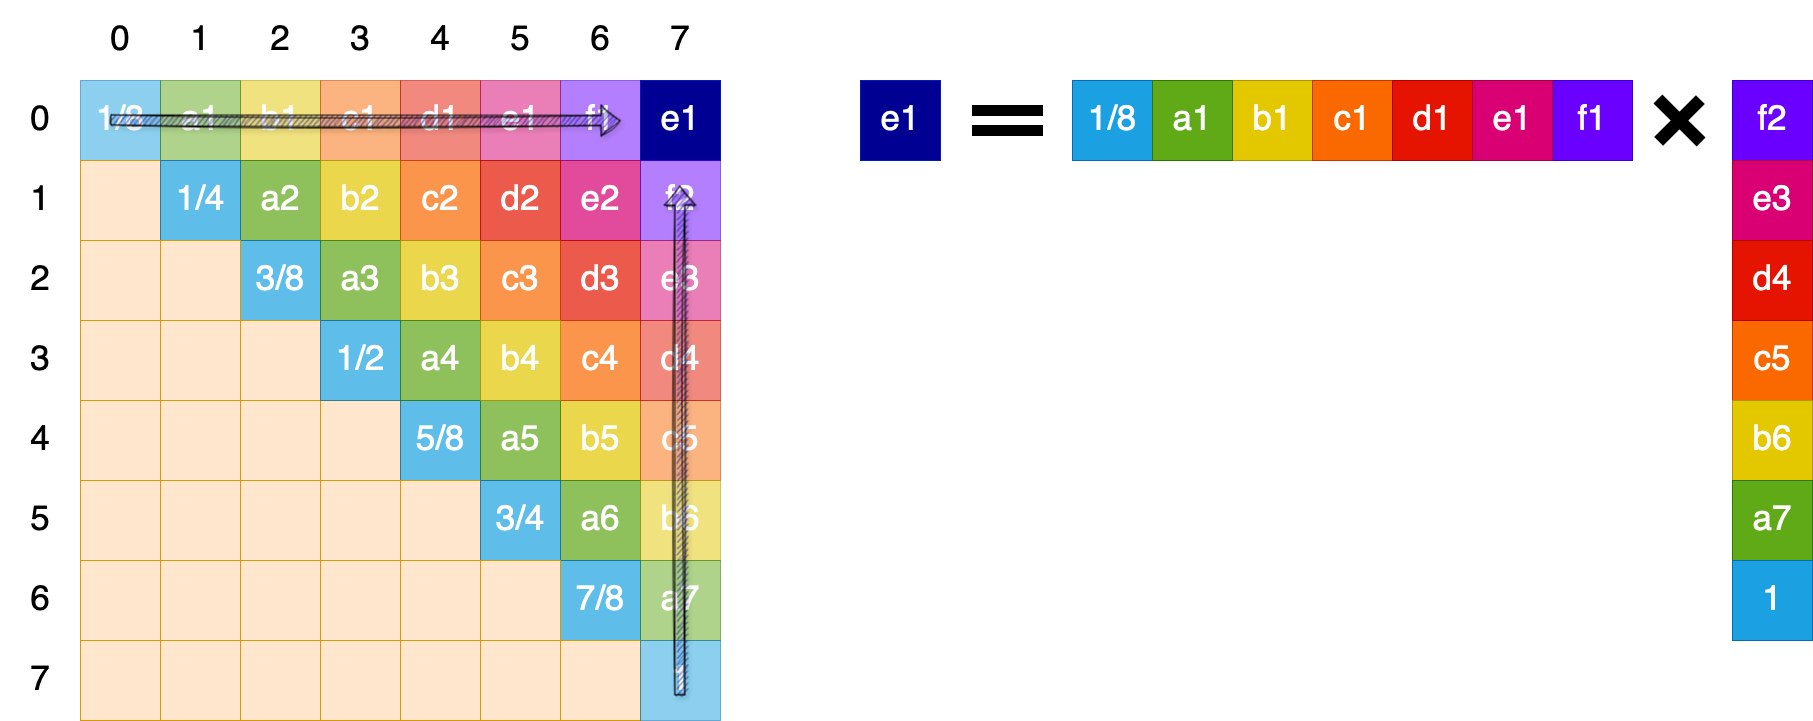
\includegraphics[scale=0.25]{img/Introduction/WaveFrontExample.png}
    
    \caption{Example of a 8x8 Matrix generated using the Wavefront Computation}
\end{figure}

\section*{Sequential Implementation}
We first develop a sequential solution to the Wavefront problem in order to identify initial optimizations and find potential parallelization opportunities. The simplest approach is to compute the diagonals sequentially, starting from the first after the major diagonal and ending with the last. Each diagonal has one less element than the previous, and computation on the next diagonal begins only after completing the current one. A basic pseudocode is shown in Algorithm \ref{Algo1}.  

\begin{algorithm}
\begin{algorithmic}
% We assume the major diagonal has index 0, so we start at index 1
\FOR{diag = 1 \textbf{to} matrix\_length - 1}
    \FOR{elem = 1 \textbf{to} diag\_length}
        \STATE Compute(elem)
    \ENDFOR
\ENDFOR
\end{algorithmic}
\caption{Basic Wavefront Sequential Pattern}
\label{Algo1}
\end{algorithm}


\subsection*{The SquareMatrix class}
\par 
In all implementations, the square matrix is represented by the custom \texttt{SquareMatrix} class. The matrix data is stored internally in a \texttt{std::vector<double>} of size $n \times n$, where $n$ is the number of rows and columns. By using a single vector instead of a \texttt{std::vector<std::vector<double>>}, we optimize both storage and efficiency.

\par The class provides methods to store and retrieve elements using row and column indices, hiding the underlying implementation to the user. Given a matrix \texttt{mtx} of type \texttt{SquareMatrix}, then an element is indexed as follows:
\begin{equation}
    \forall i \in [0, n - 1]. \forall j \in [0, n - 1]. mtx[i][j] = data[(i * n) + j]
\end{equation}

By offering methods that avoid the need to explicitly write the above formula we prevent potential bugs caused by typos when applying it multiple times in the project.

\par Additionally, the class features the method \texttt{InitializeMatrix} which sets the values of the major diagonal according to the project's requirements.

\begin{figure}[h]
    \centering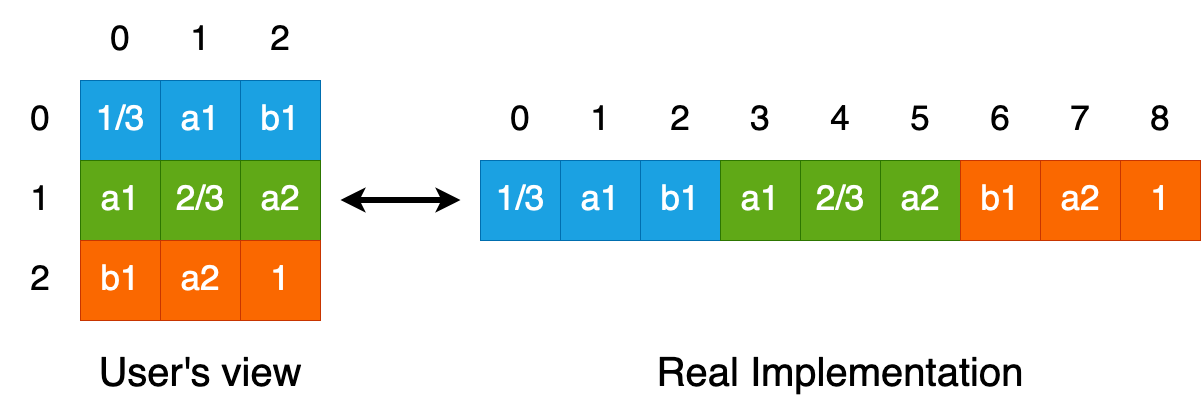
\includegraphics[scale=0.35]{img/Sequential Implementation/SquareMatriximpl.drawio.png}
    
    \caption{How the user sees a square matrix and its real implementation}
\end{figure}

\subsection*{Cache Optimization}
When computing an element of an upper diagonal, we need to calculate the dot product of its associated row and column vectors. Since the matrix is stored in a single \texttt{std::vector<double>}, elements are stored contiguously by rows. As a result, when accessing a row vector, the processor can take advantage of the locality of reference principle, storing adjacent elements in cache and optimizing retrieval during the dot product computation.
\par To achieve similar efficiency for column vectors, we can utilize the unused lower-triangular part of the matrix. Since all cells below the major diagonal are empty and unused in the Wavefront pattern, we can copy the values of the upper-triangular columns into the transposed rows of the lower-triangular part, such that:

\begin{equation}
    \forall i \in [0, n - 1]. \forall j \in [0, n - 1]. mtx[i][j] = mtx[j][i]
\end{equation}

By retrieving elements of the column vector in their corresponding lower-triangular row, we both utilize wasted space in the matrix and let the processor benefit from the locality of reference for both vectors, making the dot product more efficient.

\par To facilitate this process, the \texttt{SquareMatrix} class provides the method \texttt{SetValue(row, col, val)}, which stores the value in both the original and transposed positions within the matrix.

\begin{figure}[h]
    \centering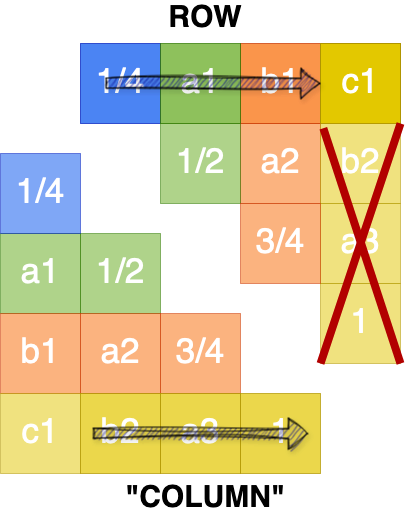
\includegraphics[scale=0.35]{img/Sequential Implementation/Locality_of_reference.drawio.png}
    
    \caption{Example of a dot product computation for the element \texttt{c1} in a 4x4 Matrix}
\end{figure}

\subsection*{Asymptotic Complexity}
For an $n \times n$ matrix, the asymptotic complexity of a Wavefront computation is determined by the processing of all upper diagonals. The $i^{th}$ diagonal has a length of $n - i$, which is equal to the number of elements to compute. Each element of a diagonal requires a dot product between vectors of length $n - i - 1$ and the application of the cube root to the result. Assuming both the cost of multiplying two elements and applying the cube root is $\mathcal{O}(1)$, then:

\begin{itemize}
    \item \textbf{Complexity of computing an element of a diagonal = } $k \times \mathcal{O}(1) + \mathcal{O}(1) = \mathcal{O}(k)$ where $k$ is the length of the vectors. 

    \item \textbf{Complexity of computing all elements of one diagonal =} $z \times \mathcal{O}(z-1) = \mathcal{O}(z^{2})$ where $z$ is the length of the diagonal.

    \item \textbf{Overall complexity = } $n-1 \times \mathcal{O}((n-1)^{2}) = \mathcal{O}(n^{3})$ where $n$ is the length of the matrix.
\end{itemize}

\subsection*{Measurements}
A C++ implementation of the sequential approach stored in \textit{``src/sequential.cpp''} has been developed to study its time complexity compared to the more efficient parallel algorithms introduced in the following sections. All project code was tested on the \textit{"spmcluster.unipi.it"} compute cluster at the University of Pisa, using various matrix sizes. Each test was run five times per matrix size, and the tables present the average results for each size.

\begin{figure}[h]
    \centering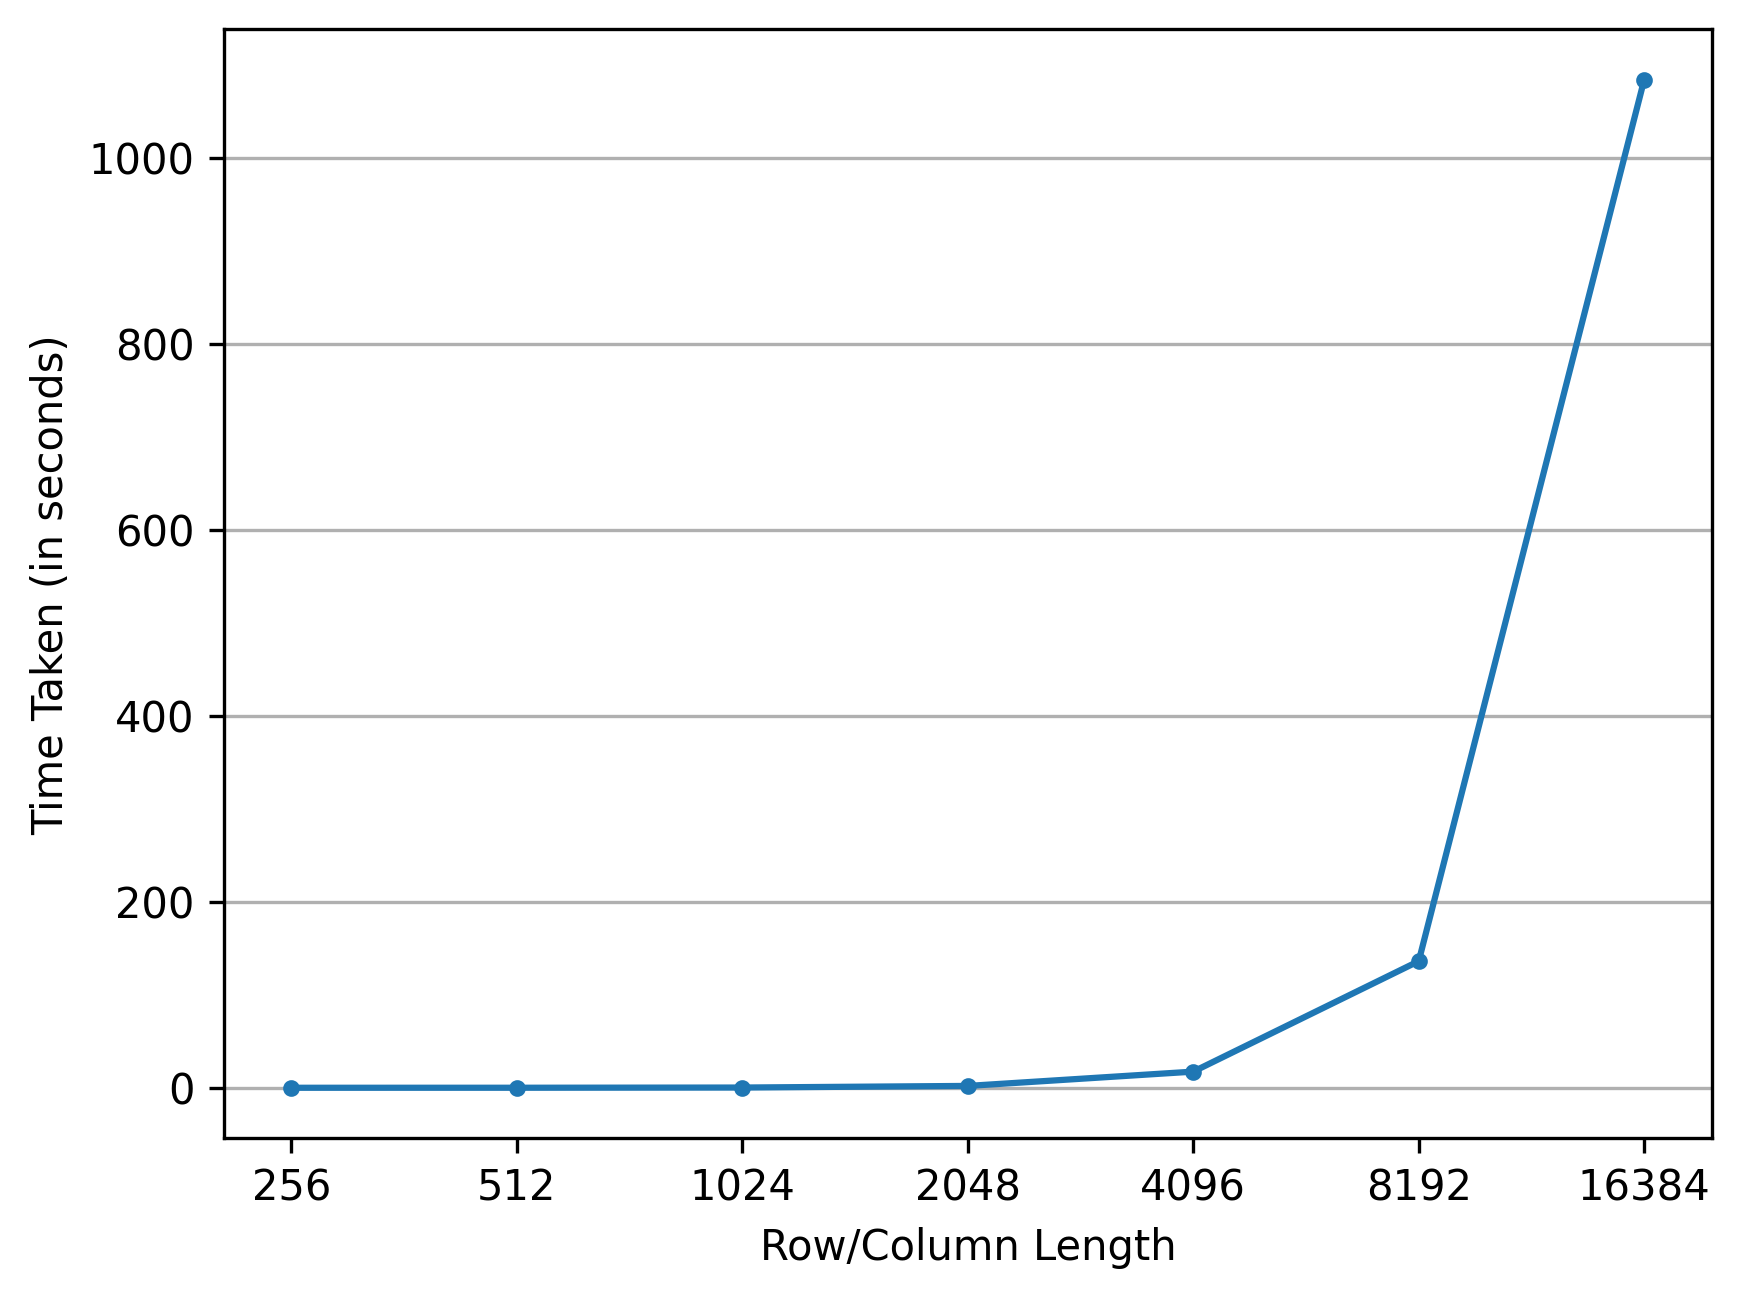
\includegraphics[scale=0.50]{img/Sequential Implementation/sequential_graph.png}
    \caption{Time measurements in seconds of the sequential C++ version of the algorithm.}
\end{figure}


\section*{FastFlow Implementation}
The first parallel implementation uses the \texttt{FastFlow C++} library, developed by the \textit{Universities of Pisa} and \textit{Turin}. The library is designed for multi/many-core CPUs and distributed systems. Each application is interpreted as a directed graph, where each node represents a concurrent processing unit in a shared-memory environment. The library provides basic building blocks and high-level patterns for common parallel computation schemes. For this project, we used the \texttt{Farm} parallel building block.

\par This version of the algorithm improves on the sequential approach by parallelizing the computation of each diagonal. Since the elements within a diagonal rely on different row and column vectors, they can be computed independently. This enables efficient use of shared memory, as threads can safely access the same matrix without race conditions. Each thread is assigned an equal (or nearly equal) portion of elements to compute. After all elements of a diagonal are processed, the algorithm advances to the next one. Threads must wait for the completion of the current diagonal before proceeding to the next. A basic pseudocode of the computation of each thread is shown in Algorithm \ref{Algo2}.

\begin{algorithm}
\begin{algorithmic}
% We assume the major diagonal has index 0, so we start at index 1
\FOR{diag = 1 \textbf{to} matrix\_length - 1}
    \STATE chunk\_size = $\lceil diag.length / num\_threads \rceil$
    \STATE Compute(chunk\_size elements)
    \STATE Waits for other threads to finish their part of the diagonal
\ENDFOR
\end{algorithmic}
\caption{Wavefront Pattern for a single thread of the Farm}
\label{Algo2}
\end{algorithm}

\subsection*{The Farm Building Block}
The key challenge in implementing Algorithm \ref{Algo2} is ensuring that threads know when to start processing their part of elements of the next diagonal. To ensure all threads have completed their current task before moving forward, this project employs the Farm high-level pattern. The Farm pattern consists of a pool of \texttt{Workers} coordinated by an \texttt{Emitter}. The \texttt{Emitter} signals the \texttt{Workers} to begin computation on the next diagonal by sending a token, which identifies the specific chunk of elements they have to process. Each \texttt{Worker} uses the token to determine its assigned elements, processes them, and then sends the token back to the \texttt{Emitter} via a feedback channel. Once the \texttt{Emitter} receives all the tokens back, it redistributes them to the \texttt{Worker}s to initiate the next diagonal's computation. Notably, the \textit{Emitter} also acts as a \texttt{Worker}, processing its chunk of elements after dispatching the tasks and before receiving them back. 

\begin{figure}[h]
    \centering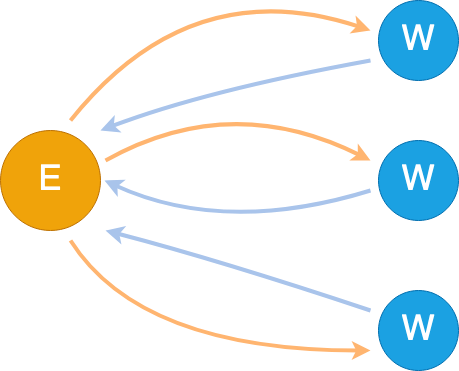
\includegraphics[scale=0.35]{img/FastFlow/Farm_graph.drawio.png}
    
    \caption{Graphical representation of the Farm.}
\end{figure}

\subsection*{Static Chunk Size vs Dynamic Chunk Size}
For each diagonal, the length is not always a multiple of the number of nodes available. In such cases, we round up the division to the nearest integer using the standard C++ function \texttt{std::ceil}. However, this can result in the last Worker receiving fewer elements than the others, or in the worst case, some Workers might receive no elements at all and not contribute to the computation.

A possible workaround is to determine the chunk size dynamically, recalculating it each time a task is sent. The dynamic chunk size is computed as:
\[
    dynamic\_chunk\_size = \lceil {remaining\_elements\_to\_send / remaining\_workers\_with\_no\_task}\rceil
\]
Although this approach requires slightly more computation compared to static case, it ensures a more even distribution of elements. However, if the number of elements in a diagonal is smaller than the number of nodes, some nodes will still remain inactive.

Theoretically the dynamic approach seems to be better than the static method, however when comparing the two in our measurements, as Figure \ref{FF_Chunk} shows, using a dynamic chunk size proves slower. This slowdown occurs probably because the overhead of managing communication between all \texttt{Workers} outweighed the marginal decrease in elements per \texttt{Worker}. Therefore, the algorithm defaults to using static chunk sizing, with the dynamic approach available as an optional alternative through the use of the guard \texttt{DYNAMIC\_CHUNK}.

\begin{figure}[h]
    \centering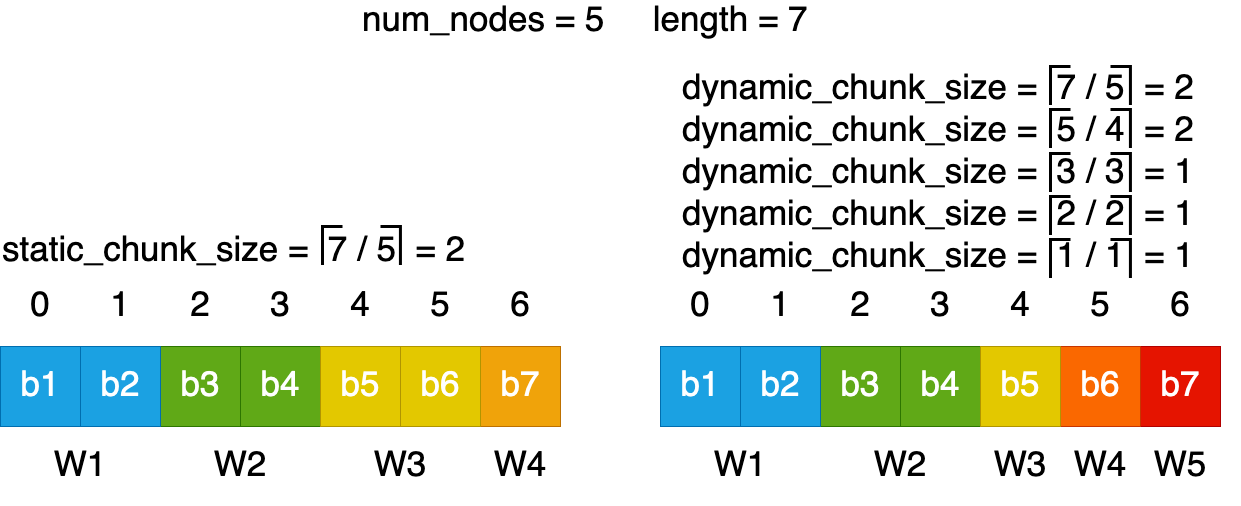
\includegraphics[scale=0.20]{img/FastFlow/Static_vs_Dynamic.drawio.png}
    
    \caption{Example of the distribution of Workers using static and dynamic chunk size.}
\end{figure}

\subsection*{The DiagInfo class}
Each node needs to track the current diagonal it is processing and its length to determine which elements to compute. Instead of requiring each node to update a local copy of these values with each new task, the information is shared in the object of custom type \texttt{DiagInfo}. Only the \texttt{Emitter} has the responsibility to update before starting work on the next diagonal, through the \texttt{PrepareNextDiagonal()} method. The \texttt{Worker}s simply read from it during their computations.

\subsection*{Farm Limitation}
Another potential parallel optimization lies in the dot product computation. Instead of calculating it element by element, the row and column vectors could be divided into segments, with each segment handled by a different thread. The partial results would then be summed to produce the final dot product. While this idea is appealing, it is impractical in our current approach. As the computation progresses, the diagonals become smaller, eventually having fewer elements than available \texttt{Worker}s. For example, the last diagonal has only one element, leaving most \texttt{Worker}s idle. Unfortunately, in \texttt{FastFlow}'s \texttt{Farm} building block, \texttt{Worker}s cannot directly communicate, so coordinating this task would require extensive communication managed by the \texttt{Emitter}, leading to inefficiencies.

\subsection*{Asymptotic Complexity}
Assume the cost of communication between the \texttt{Emitter} and one \texttt{Worker} is a constant $\mathcal{O}(c)$ with $c > 0$, the complexity simplifies to:

\begin{itemize}
    \item \textbf{Complexity of sending tasks to each Worker =} $num\_workers \times \mathcal{O}(num\_workers \times c)$

    \item \textbf{Complexity of computing all elements of one diagonal =} $ \mathcal{O}(num\_workers \times c) + \mathcal{O}(\max{chunk\_size}) = \mathcal{O}(num\_workers \times c) + \mathcal{O}(\lceil n-1 / num\_threads \rceil)$ where $n$ is the length of the matrix.

    \item \textbf{Overall complexity = } $n-1 \times (\mathcal{O}(num\_workers \times c) + \mathcal{O}(\lceil n-1 / num\_threads \rceil) ) =\mathcal{O}((n - 1) \times num\_workers \times c) + \mathcal{O}((n-1)^{2} / num\_threads)$ where $n$ is the length of the matrix.
\end{itemize}

\subsection*{Measurements}
A \texttt{C++} implementation of the \texttt{FastFlow} approach is implemented in \textit{src\_parallel\_fastflow.cpp}. The program takes the matrix size and the number of threads as arguments. By passing $m$ and $n$, the process creates one \texttt{Emitter} and $n - 1$ \texttt{Workers} to handle a matrix of size $m \times m$. When compiling the project using the CMake configuration files, it will generate two executables: one using static chunk sizes and the other using dynamic chunk sizes. Both versions have been tested on the \textit{``spmcluster.unipi.it''} compute cluster with various thread counts and matrix sizes. It is important to note that while each node in the \textit{spmcluster} is advertised as having $32$ cores, it actually consists of $16$ physical cores, with the remaining ones being virtual cores (\textit{hyperthreaded}).
\par 
The speedup graph in Figure \ref{FF_Speedup} demonstrates that using more threads results in greater performance gains. However, the efficiency graph in Figure \ref{FF_Efficiency} reveals that as the number of threads increases, efficiency diminishes, indicating that the overhead associated with managing additional threads becomes more and more large. 

\begin{figure}[h!]
    \centering
    % First row: Two images adjacent
    \begin{minipage}[t]{0.49\textwidth}
        \centering
        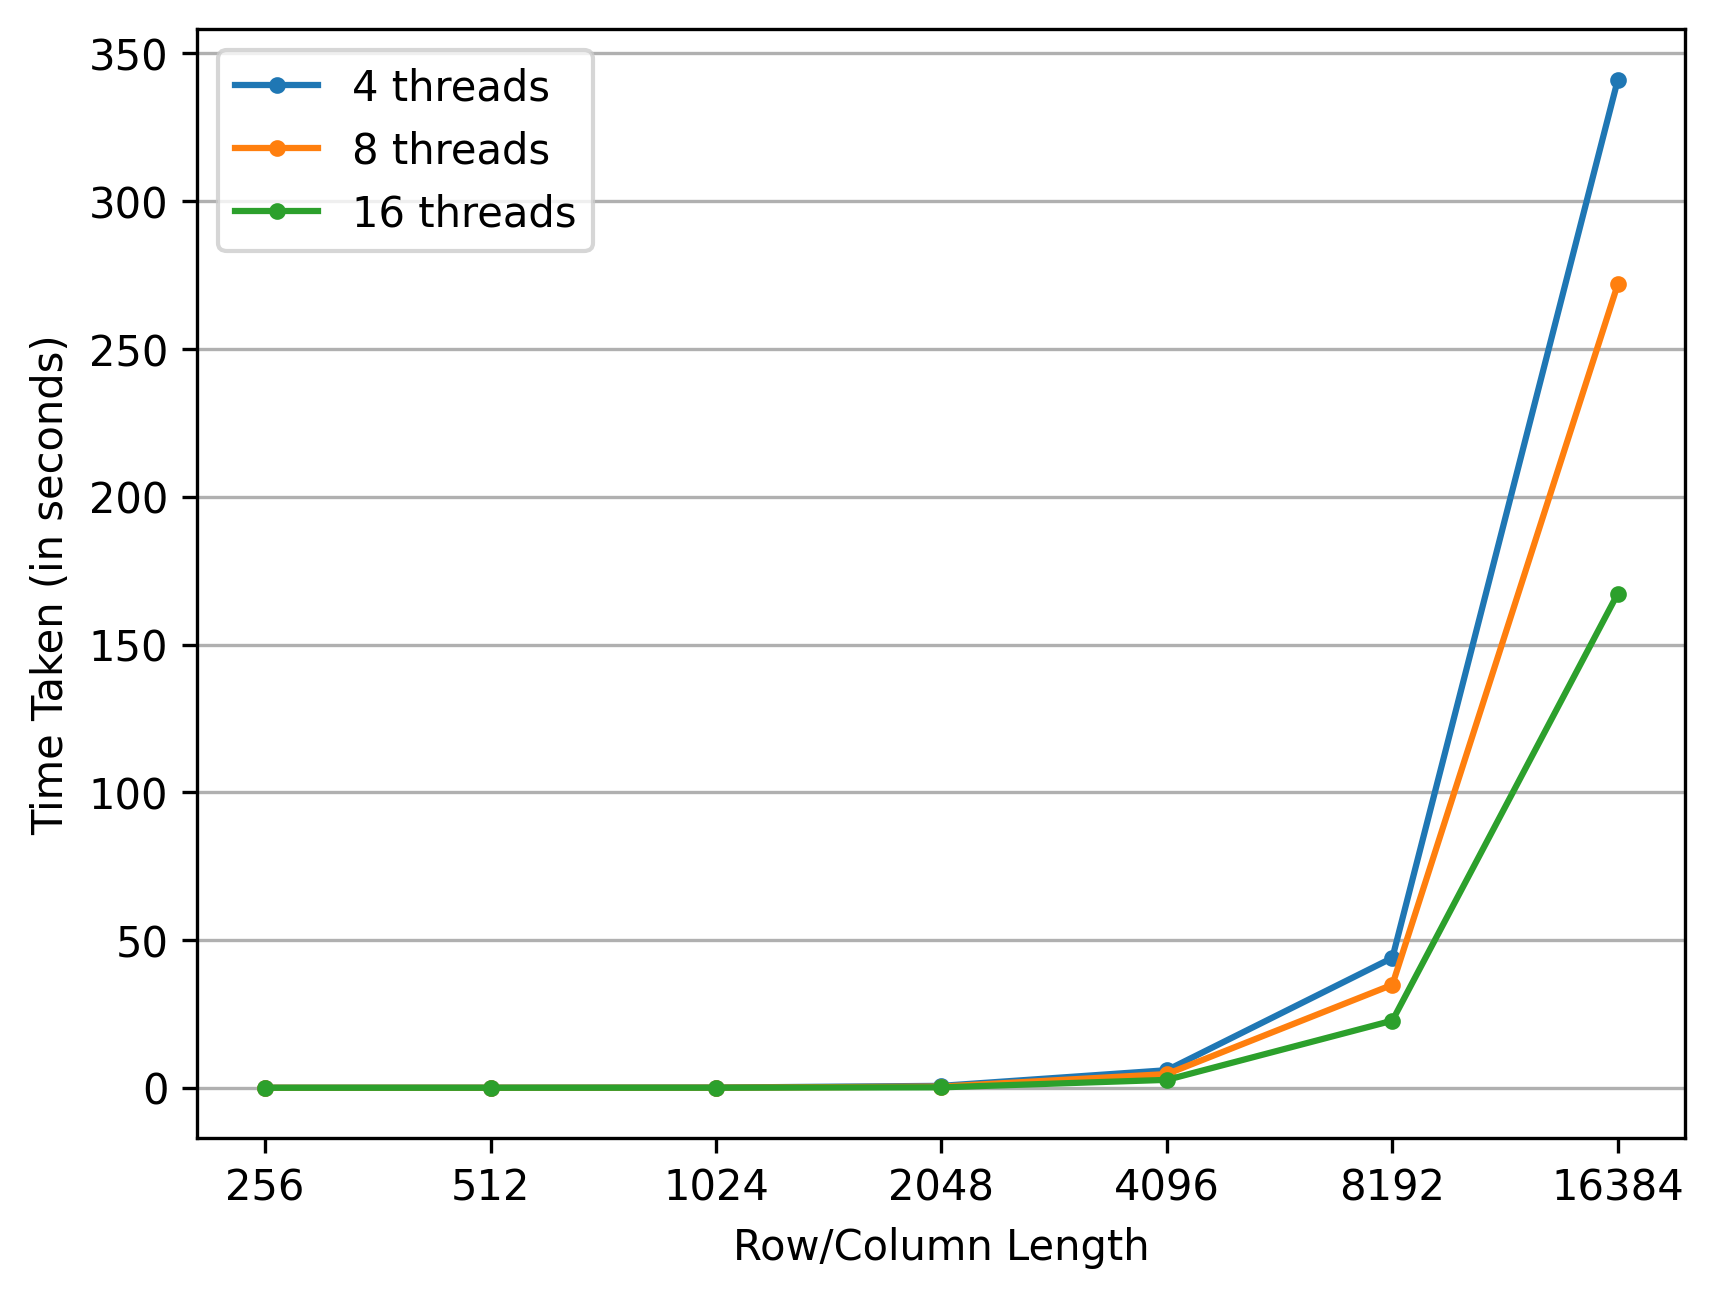
\includegraphics[width=\textwidth]{img/FastFlow/ff_static_graph.png}
        \caption{FastFlow Strong Scaling comparison.}
        \label{FF_Strong_scaling}
    \end{minipage}
    \hfill
    \begin{minipage}[t]{0.49\textwidth}
        \centering
        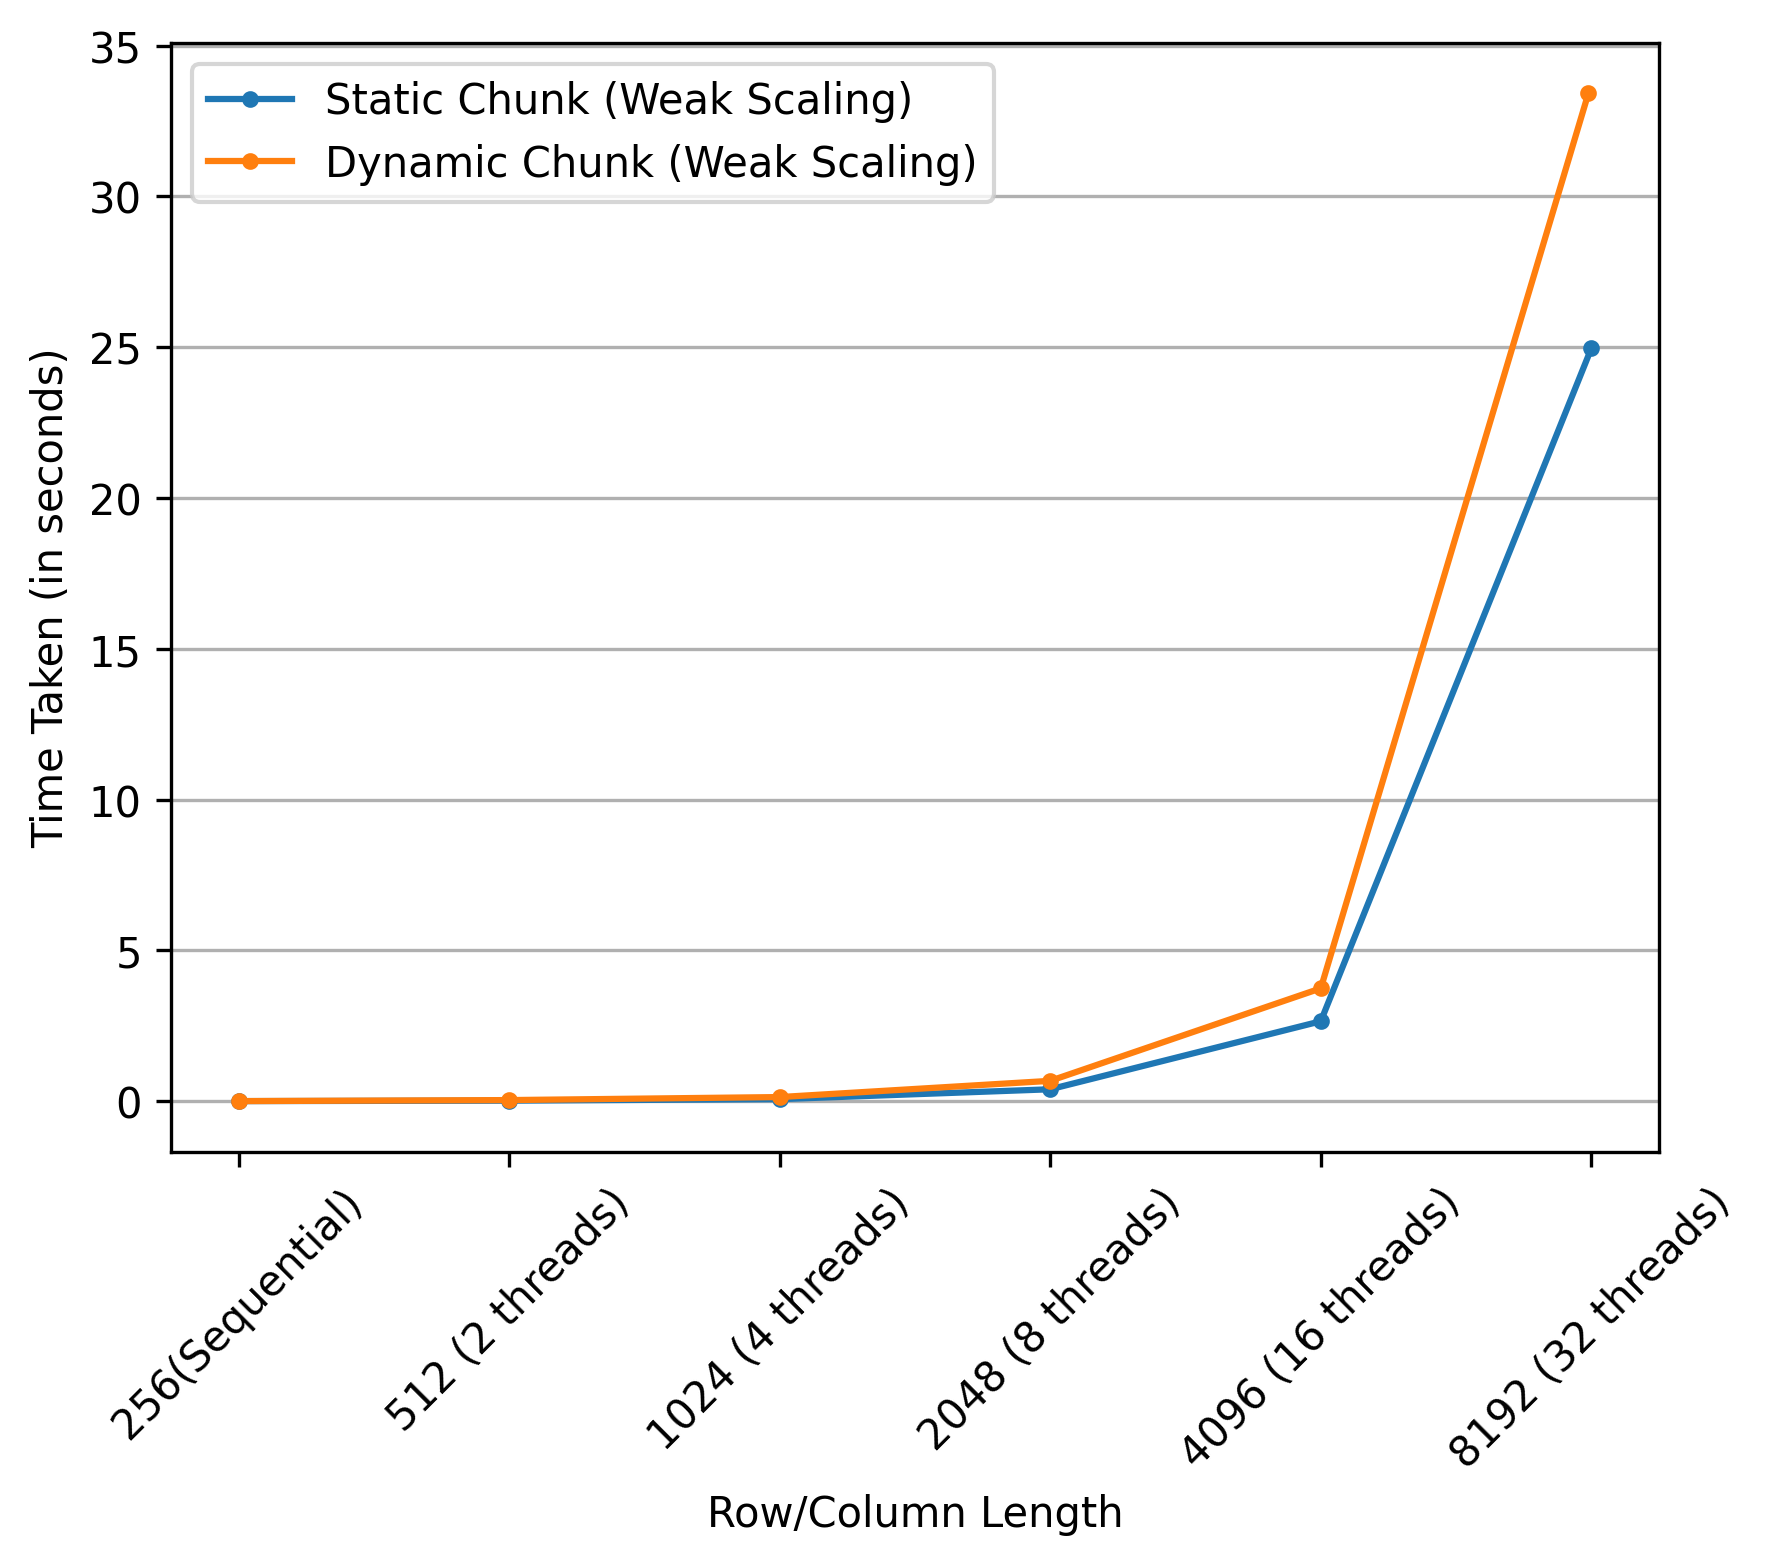
\includegraphics[width=\textwidth]{img/FastFlow/ff_static_vs_dynamic.png}
        \caption{FastFlow Weak scaling comparison.}
        \label{FF_Chunk}
    \end{minipage}
    
    % First row: Two images adjacent
    \begin{minipage}[t!]{0.49\textwidth}
        \centering
        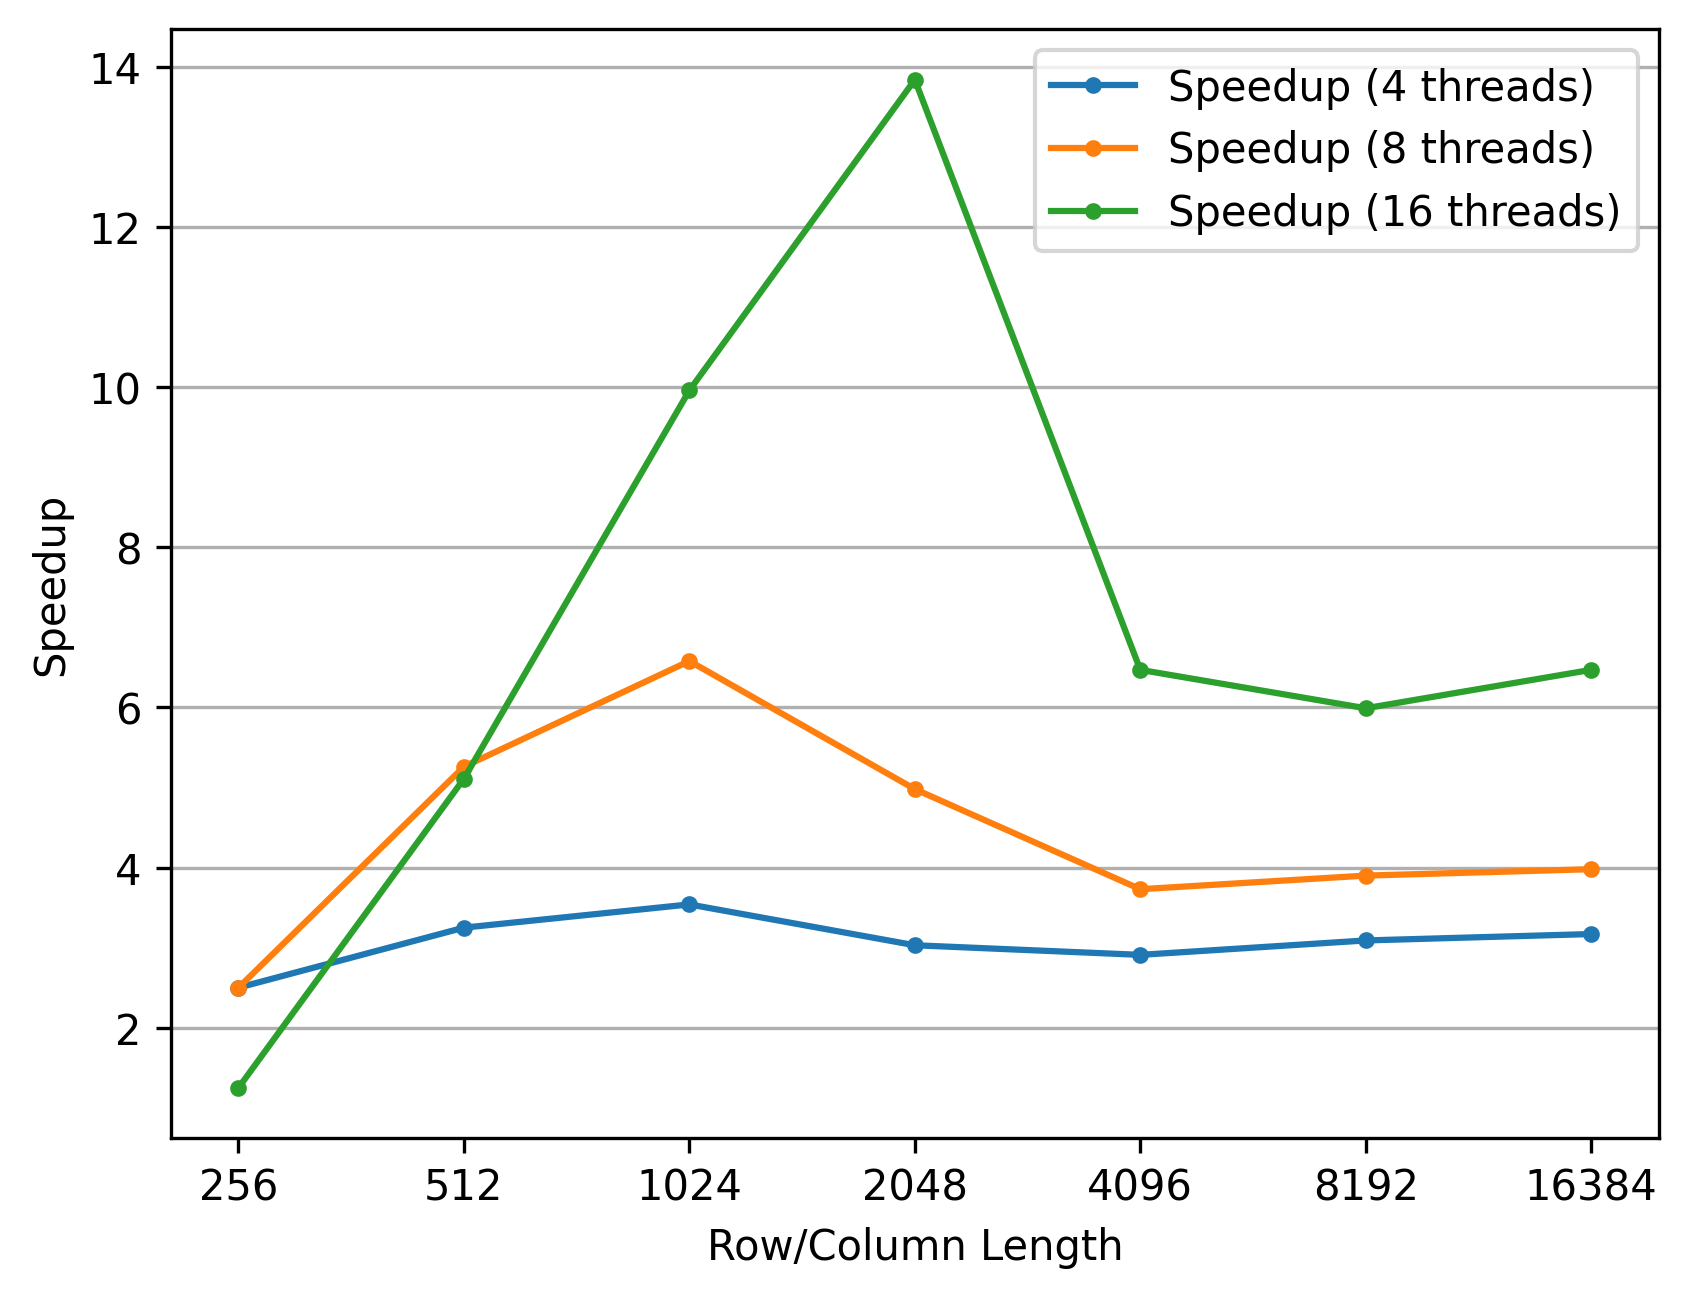
\includegraphics[width=\textwidth]{img/FastFlow/ff_speedup.png}
        \caption{FastFlow Speedup comparison.}
        \label{FF_Speedup}
    \end{minipage}
    \hfill
    \begin{minipage}[t!]{0.49\textwidth}
        \centering
        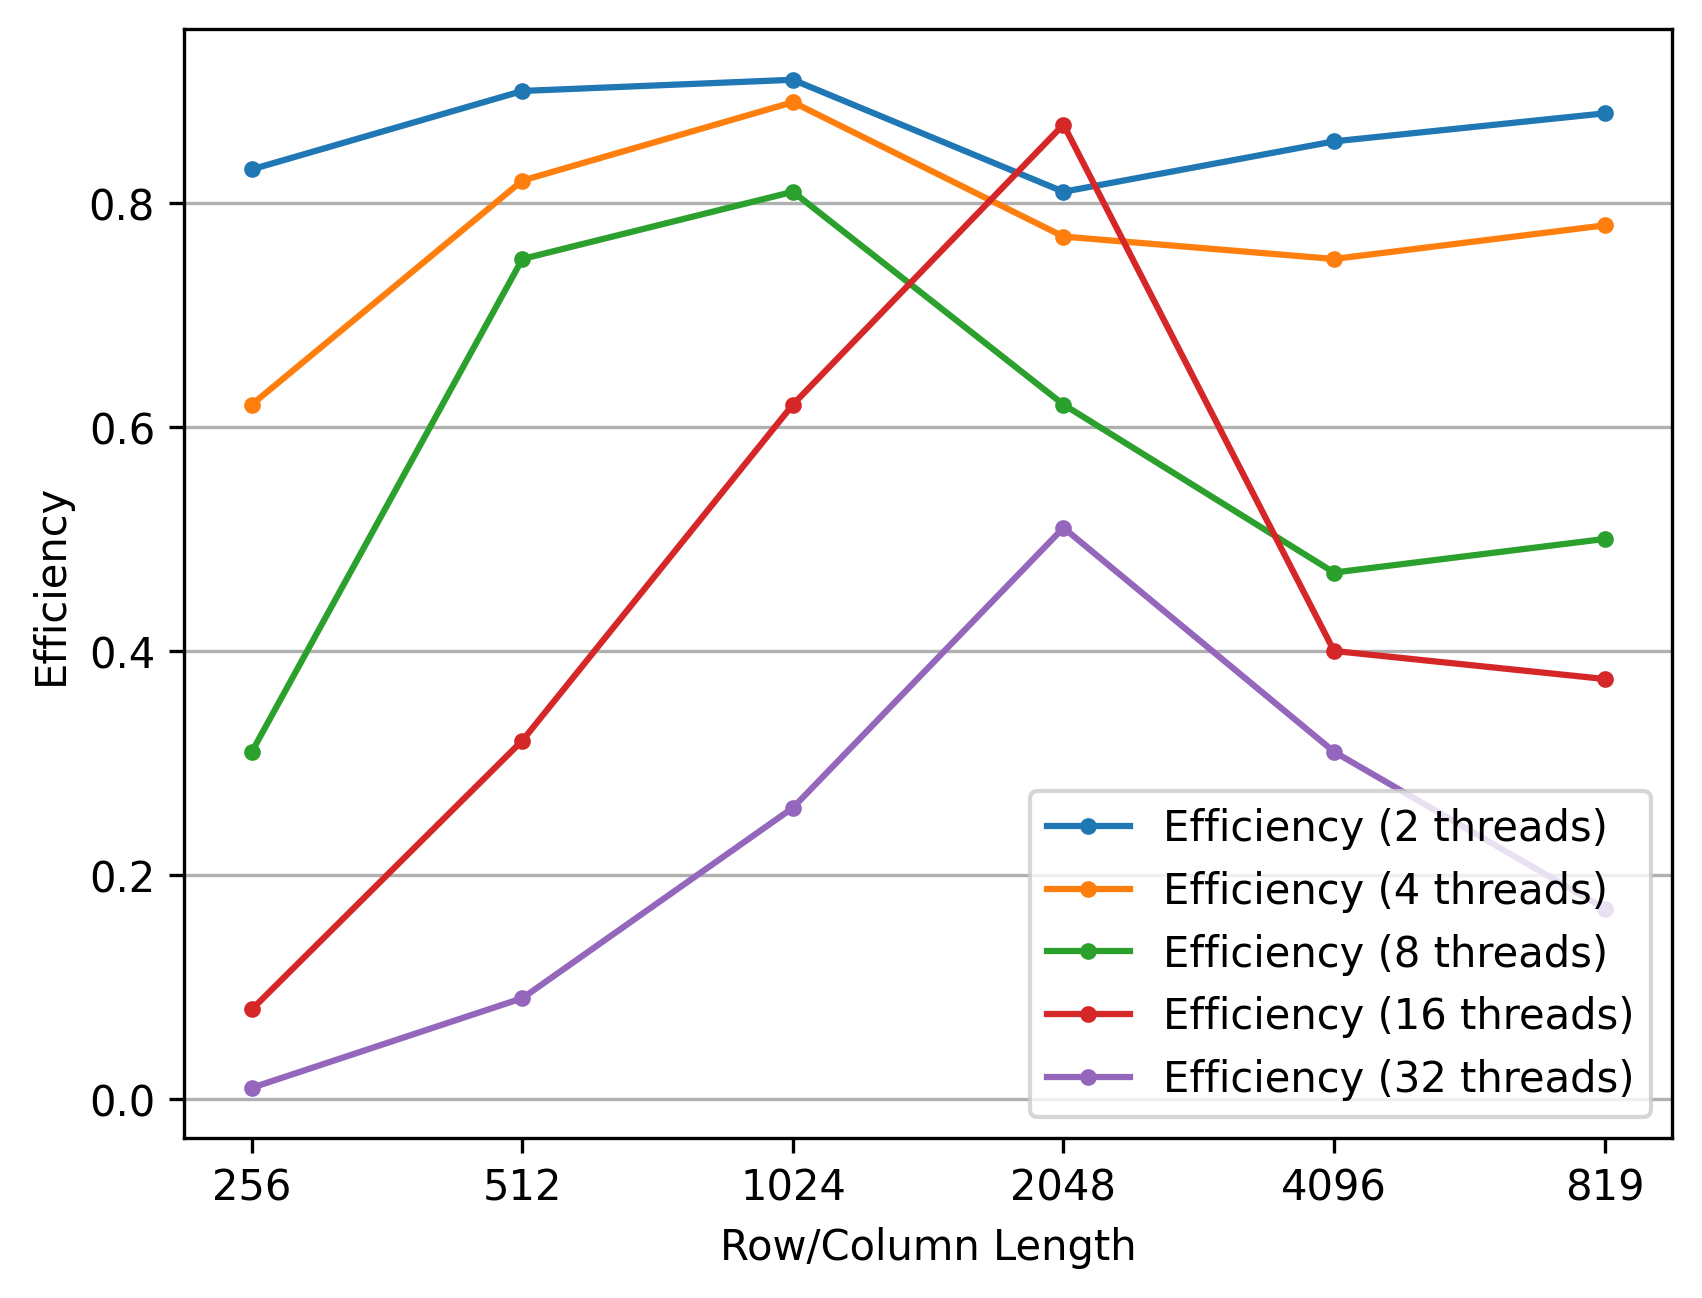
\includegraphics[width=\textwidth]{img/FastFlow/ff_efficiency.png}
        \caption{FastFlow Efficiency comparison.}
        \label{FF_Efficiency}
    \end{minipage}

    \begin{minipage}[t]{0.49\textwidth}
        \centering
        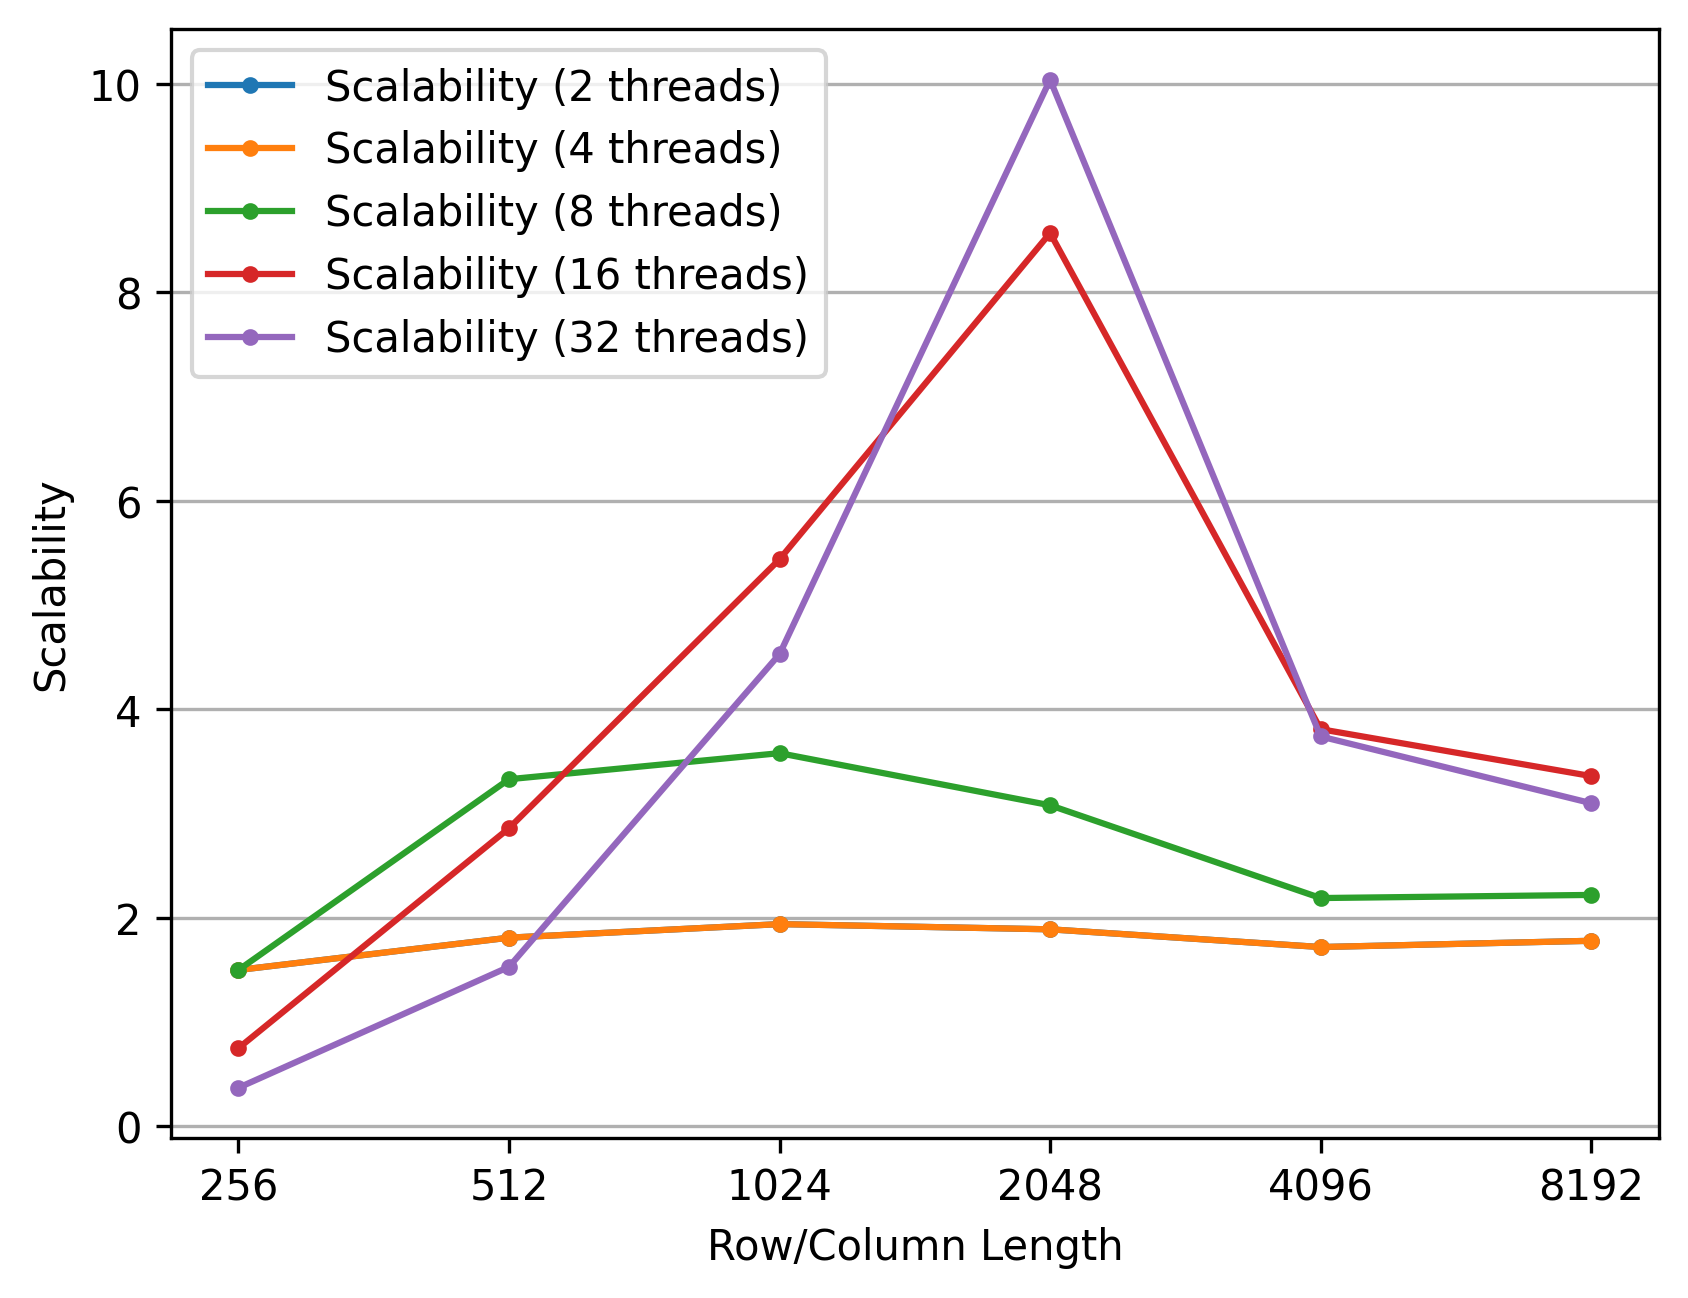
\includegraphics[width=\textwidth]{img/FastFlow/ff_scalability.png}
        \caption{FastFlow Scalability comparison.}
        \label{FF_Scalability}
    \end{minipage}
    \hfill
    \begin{minipage}[t]{0.49\textwidth}
        \centering
        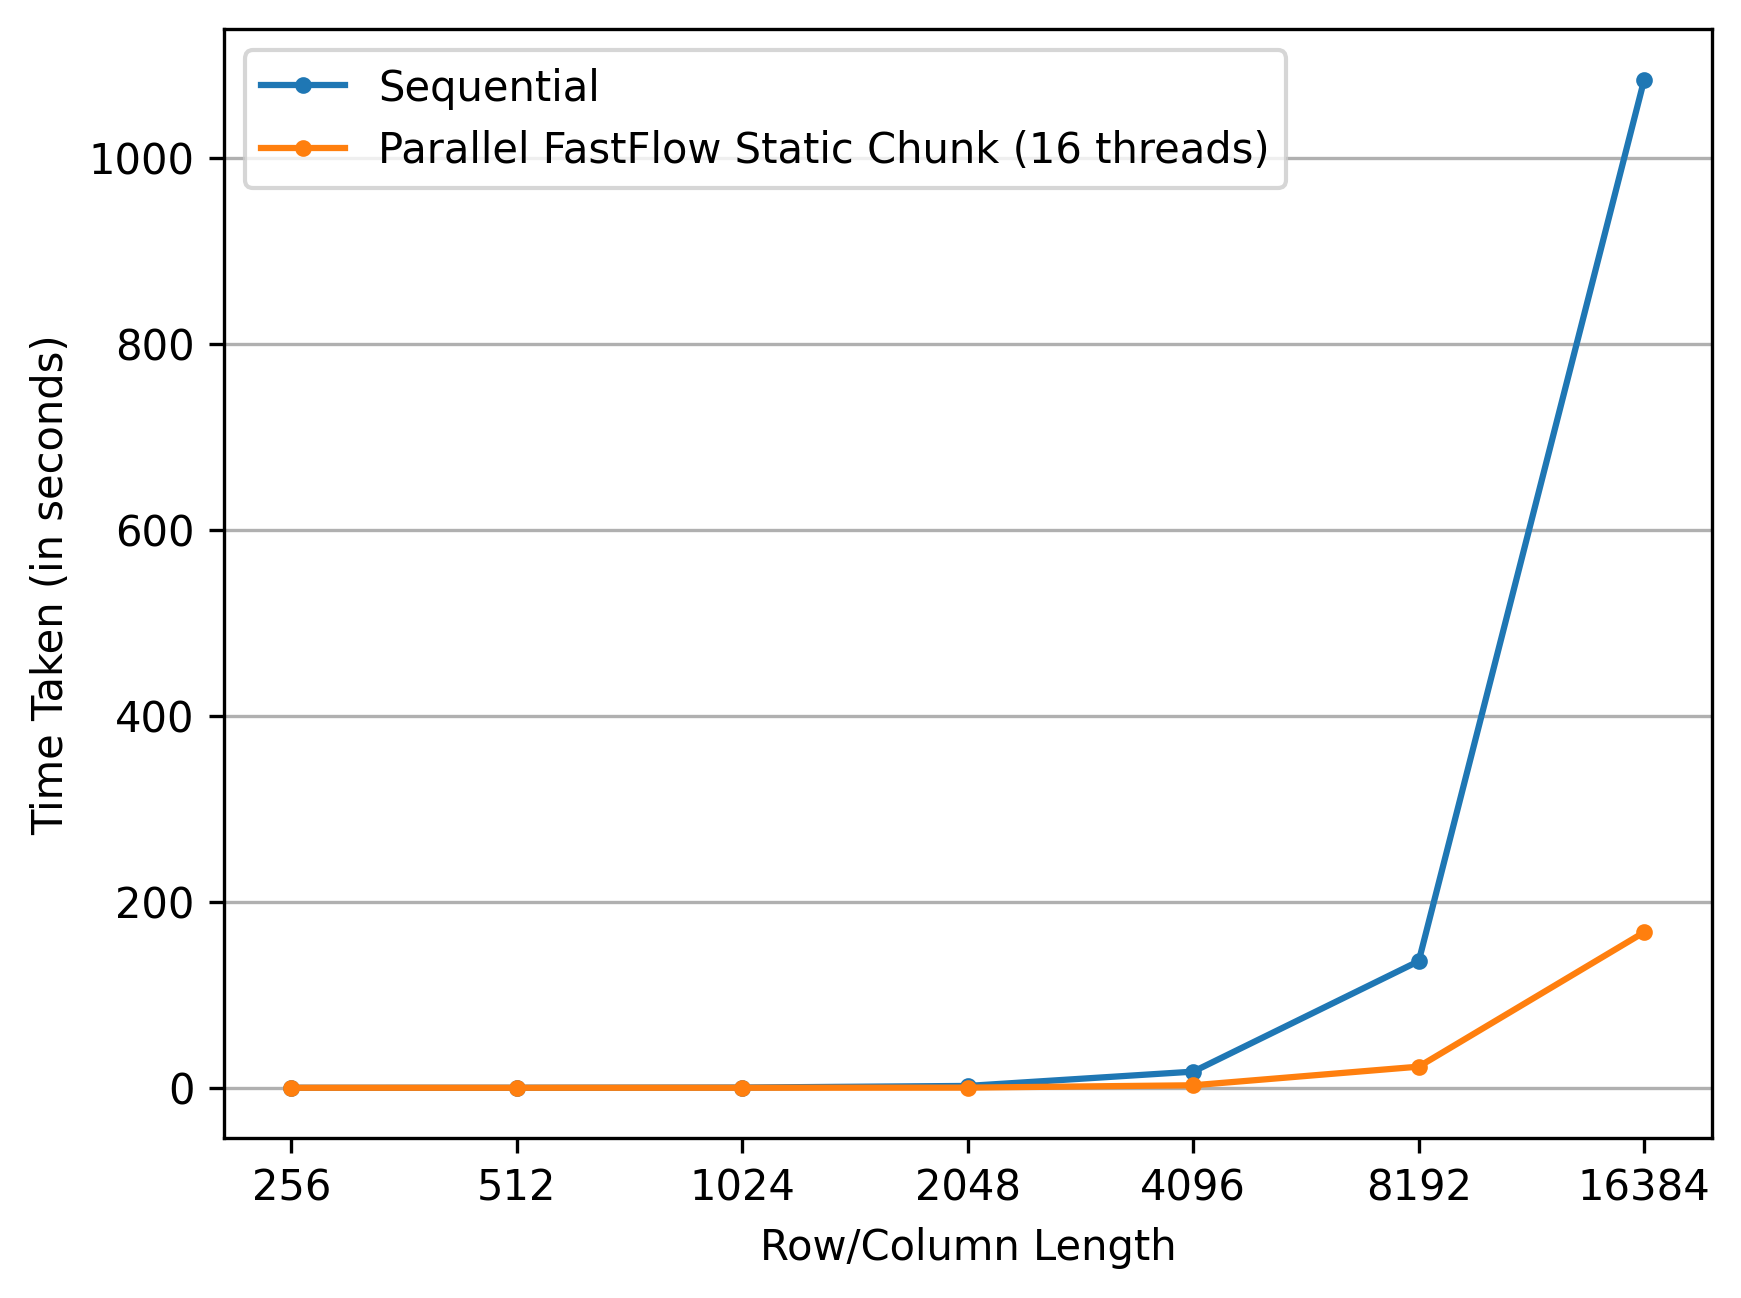
\includegraphics[width=\textwidth]{img/FastFlow/ff_sequential_vs_fastflow.png}
        \caption{Comparison between sequential and FastFlow implementations.}
        \label{FF_Sequential_vs_FastFlow}
    \end{minipage}
\end{figure}
\section*{MPI Implementation}
The second parallel implementation utilizes the \texttt{OpenMPI} and \texttt{OpenMP} \texttt{C++} libraries. \texttt{OpenMPI} is an open-source implementation of the \texttt{MPI} standard, which provides a message-passing interface to enable communication between multiple processes, often distributed across different nodes in a cluster or supercomputer. \texttt{OpenMP}, similar to \texttt{FastFlow}, simplifies parallel programming within shared-memory systems by enabling efficient use of multiple processors or cores within a single node.

\par In this version of the algorithm, \texttt{OpenMPI} handles communication between nodes, while \texttt{OpenMP} is employed inside each node to parallelize local computation. In contrast to the previous implementation, this solution operates in a distributed memory environment, where each node functions as an independent process with its own local memory. As a result, explicit communication between nodes is necessary to share data and coordinate tasks.

\subsection*{The Divide et Impera approach}

\par To optimize the balance between local computation and inter-process communication, a \textit{Divide et Impera} strategy has been employed. At the start of execution, the system consists of $n$ nodes, each of which can assume the role of either \texttt{Master} or \texttt{Supporter}. A \texttt{Master} can have up to two \texttt{Supporter}s, while each \texttt{Supporter} is associated with only one \texttt{Master}. \texttt{Master}s do not share \texttt{Supporter}s with one another.

After determining their roles and associations independently, each node computes a submatrix of the final matrix. The size of each submatrix is determined by dividing the entire matrix by the number of active processes, while the portion of elements is determined by an id associated to the node. Once a \texttt{Supporter} has completed its assigned submatrix, it sends the result to its \texttt{Master}. The \texttt{Master} then merges the received results with its own computation.

After merging, the \texttt{Supporter}s terminate their execution, decreasing the number of active processes. The remaining \texttt{Master}s redetermine their roles, potentially becoming \texttt{Supporter}s, and the process iterates. The algorithm concludes when only one node remains, referred to as the \texttt{Last} node, which computes the final portion of the matrix and completes the execution. A pseudocode describing a node behaviour of this approach is shown in Algorithm \ref{Algo3}.

\begin{algorithm}
\begin{algorithmic}
\WHILE{TRUE}
    \STATE role = DetermineMyRole();
    \STATE ComputeMySubMatrix();
    \IF{I am a Master or a Supporter}
        \STATE MergeMatrices();
    \ENDIF
    \IF{I am a Supporter or the Last active node}
        \STATE EndExecution();
    \ENDIF
\ENDWHILE
\end{algorithmic}
\caption{Wavefront Pattern for a node in the MPI algorithm}
\label{Algo3}
\end{algorithm}


\begin{figure}[h]
    \centering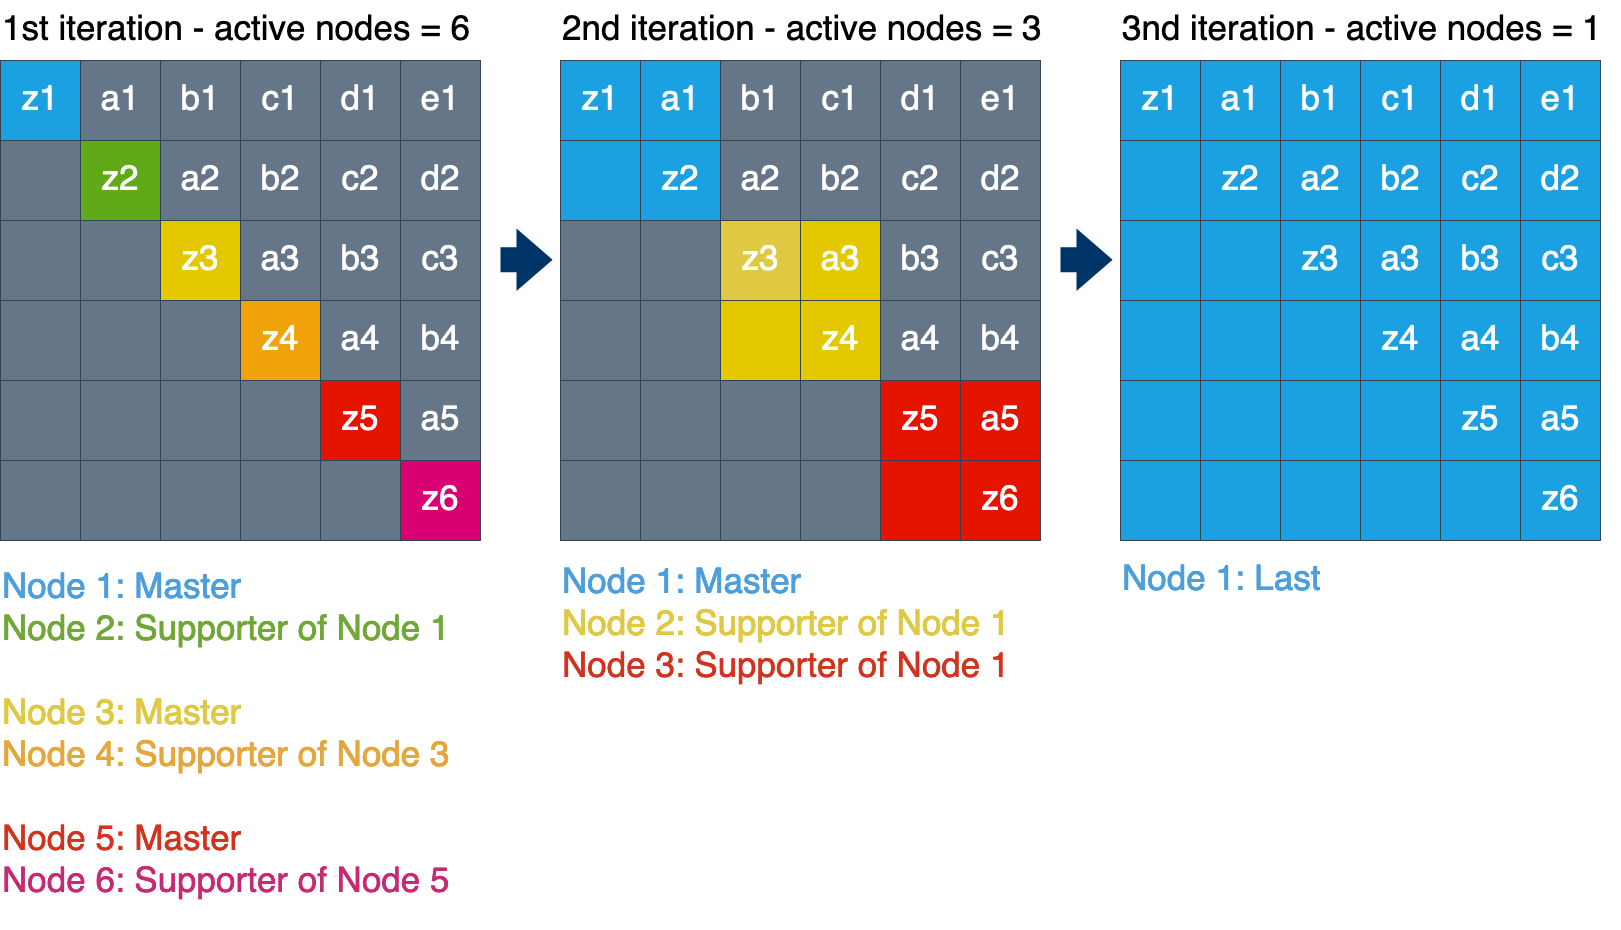
\includegraphics[scale=0.30]{img/MPI/DivideEtImpera.drawio.png}
    
    \caption{Example of an execution of the MPI parallel algorithm}
\end{figure}


\subsection*{OpenMP usage}
\texttt{OpenMP} is utilized within a node to compute its submatrix. Previous implementations have shown that both the computation of elements along the same diagonal and the dot product computation for individual elements can be parallelized. Both parallelization are achieved using separate \texttt{Parallel For} constructs. In the case of the dot product computation, since the local multiplications needs to be summed to obtain the final result, the \texttt{reduction} paradigm is employed to combine these local copies into a final value. Additionally, \texttt{OpenMP} is used by both roles when merging their matrices. Because the rows to be copied are distinct, these communications can be executed concurrently.

\subsection*{Determining the role of a Node}
As previously mentioned, a node can take on one of three roles: \texttt{Master}, \texttt{Supporter}, or \texttt{Last}. The role of a node is determined at the beginning of each iteration based on its \texttt{id}, the number of active nodes, and the size of the final matrix. If the matrix size is smaller than the number of nodes, the excess nodes are removed at the start of the computation as they are not needed. The node's \texttt{id} is recalculated at each iteration: initially, it matches the \texttt{rank} assigned by \texttt{MPI}, but in subsequent iterations, it depends on the number of active nodes. \texttt{id}s begin at zero. The relation between the \texttt{rank} of a node and its \texttt{id} is the following:

\begin{equation}
    current\_id = \lceil rank / 2^{current\_iteration - 1}\rceil
\end{equation}

A \texttt{Master} node is always assigned an even \texttt{id} and must have an adjacent node. \texttt{Supporter} nodes either have an odd \texttt{id} or are even-numbered without any following nodes. Once a \texttt{Supporter} node completes its computation, it exits the Wavefront computation and waits for the program to terminate. Thus the number of active nodes at each iteration is equal to the previous one divided by two. The \texttt{Last} node is, as the name implies, the only node left in the final iteration. It has a unique role since it is the only node that does not need to merge its matrix with any other node; it computes the remaining elements and then exits the computation.

\subsection*{Communication between nodes}
After completing the computation of its sub-matrix, a node must exchange data with its partners, either sending its own results or receiving results from others. A node can communicate only with its associated \texttt{Master} or \texttt{Supporter}s. During the role determination of a node, the algorithm also identify the \texttt{rank}s of the nodes it needs to communicate with. For a \texttt{Supporter}, the node stores the rank of the \texttt{Master} in the variable \texttt{my\_master}, while for a \texttt{Master}, it stores the \texttt{rank}s of its \texttt{Supporter}s in the vector \texttt{my\_supporters}. The \texttt{MergeMatrices} method manages this communication.

\par In this method, both roles determine which rows to send or receive based on the final matrix configuration. The rows are calculated using the \texttt{Supporter} node's \texttt{id} as follows:

\begin{align*}
    first\_row &= supporter\_id \times sub\_mtx\_length \\
    last\_row &= first\_row + (sub\_mtx\_length - 1) \\
    num\_rows &= (last\_row - first\_row) + 1
\end{align*}

Next, the process identifies for each row, regarding its role, the index of the first element computed by the \texttt{Supporter}. Communication is then handled synchronously using either \texttt{MPI\_Send} or \texttt{MPI\_Recv}, depending on the role. The \texttt{std::vector<double>} containing the data is passed as a buffer, offset to the calculated index, and $lenght\_sub\_matrix$ elements are retrieved. Since each send/receive is done on a different row, the process is sped up through parallelization using the \texttt{Parallel For} construct.

This implementation still exploits the locality of reference principle storing a copy of the columns of the upper-triangular as rows of the lower-triangular part, thus these values are considered during the copy. Although it might seem beneficial to send only the necessary elements of a row, rather than copying repeating elements, this avoids the \texttt{Master} to copy manually the received elements in their transposed position on the lower-triangular matrix. 

\begin{figure}[h]
    \centering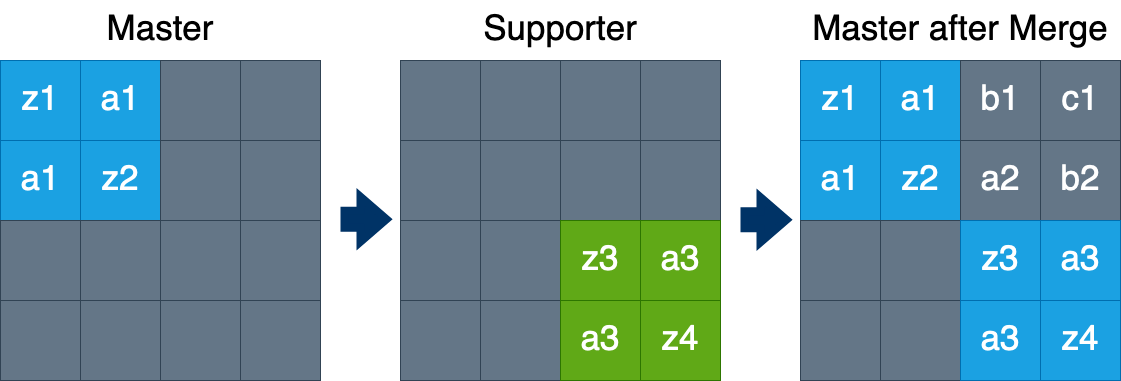
\includegraphics[scale=0.25]{img/MPI/MergeMatrix.drawio.png}
    
    \caption{Example of merging the matrices of a Master and its associated Supporter.}
\end{figure}

\subsection*{The WavefrontNode Class}
Each process spawned by \texttt{MPI} creates an instance of the \texttt{WavefrontNode} class. This class encapsulates all the methods and variables required for a node to perform the necessary computations. Upon creation, the constructor initializes essential information such as the node's \texttt{id} and \texttt{rank}, and then calls the \texttt{WaveFrontComputation()} method, which implements the pseudocode outlined in Algorithm \ref{Algo3}. By the end of the program, the node assigned the role of \texttt{Last} holds the final matrix, which is stored as a \texttt{SquareMatrix} object within itself.

\subsection*{Asymptotic Complexity}
Compared to the \texttt{FastFlow} algorithm, the asymptotic complexity of the current solution is theoretically more efficient. This is because each node computes a smaller portion of the overall matrix, and during the computation it can leverage both diagonal and dot product parallelism. Assuming the communication cost for sending/receiving  a single element of the matrix is $\mathcal{O}(1)$, and the cost for determining the node's current role is also $\mathcal{O}(1)$, then:
\begin{itemize}


    \item \textbf{Complexity of computing a single sub matrix =} $\mathcal{O}(\max{sub\_matrix\_length}) = \mathcal{O}((n-1)/ num\_nodes )$ where $n$ is the length of the matrix and $num\_nodes$ is the number of nodes employed in the pattern.

    \item \textbf{Complexity of sending/receiving a single row =} $row\_length \times \mathcal{O}(1) = \mathcal{O}(row\_length) = \mathcal{O}(n - 1)$ where $n$ is the length of the matrix

    \item \textbf{Complexity of merging matrices =} $2 \times \mathcal{O}(row\_length) = \mathcal{O}(n - 1)$

    \item \textbf{Complexity of an iteration for one node =} $ \mathcal{O}(1) + \mathcal{O}(n - 1) + \mathcal{O}((n-1)/ num\_nodes) = \mathcal{O}(n-1)$

    \item \textbf{Overall Complexity =} $ \sum_{iteration = 0}^{(n-1) / num\_nodes}{\mathcal{O}(n-1)} = \mathcal{O}(n-1)^{2}$
\end{itemize}

However, as the measurement section will demonstrate, approximating the communication is overly optimistic. In reality, for smaller matrices, the communication overhead significantly impacts the overall complexity, making it less efficient than the previous shared memory solution and in some cases even the sequential case.

\subsection*{Measurements}
The C++ implementation can be found in \texttt{src\_parallel\_mpi.cpp}. It's important to note that the program must be executed using the command \texttt{mpirun -N [number of nodes]}; otherwise, it will run sequentially. The implementation has been thoroughly tested with various matrix sizes and different numbers of nodes. Additionally, the behavior of the program has been evaluated both when dedicating an entire cluster node to a single program node and when assigning multiple program nodes to each machine in the cluster. Interestingly, assigning more than one process per node results in worse performance compared to the standard case as Figure \ref{MPI_THEADS} shows. This likely occurs because, although each process handles smaller matrices and the initial \texttt{Master-Supporter} pairs are typically assigned to processes within the same machine, resulting in lower communication overhead compared to contacting processes on different nodes, the increased overhead of managing more processes still outweighs these benefits.

\par For relatively small matrices (up to 1024 in length), the execution is slower than previous approaches due to communication overhead. Our tests showed minimal optimization when increasing the number of nodes from four to eight. As illustrated in Figure \ref{MPI_Speedup}, even though each node handles smaller matrices, the communication overhead of managing additional nodes negates any potential gains. Overall, in the matrices we tested, the \texttt{FastFlow} implementation outperforms \texttt{MPI}, obviously, as accessing the matrix within a shared memory environment is significantly faster than passing submatrices.

\begin{figure}[h!]
    \centering
    % First row: Two images adjacent
    \begin{minipage}[t]{0.49\textwidth}
        \centering
         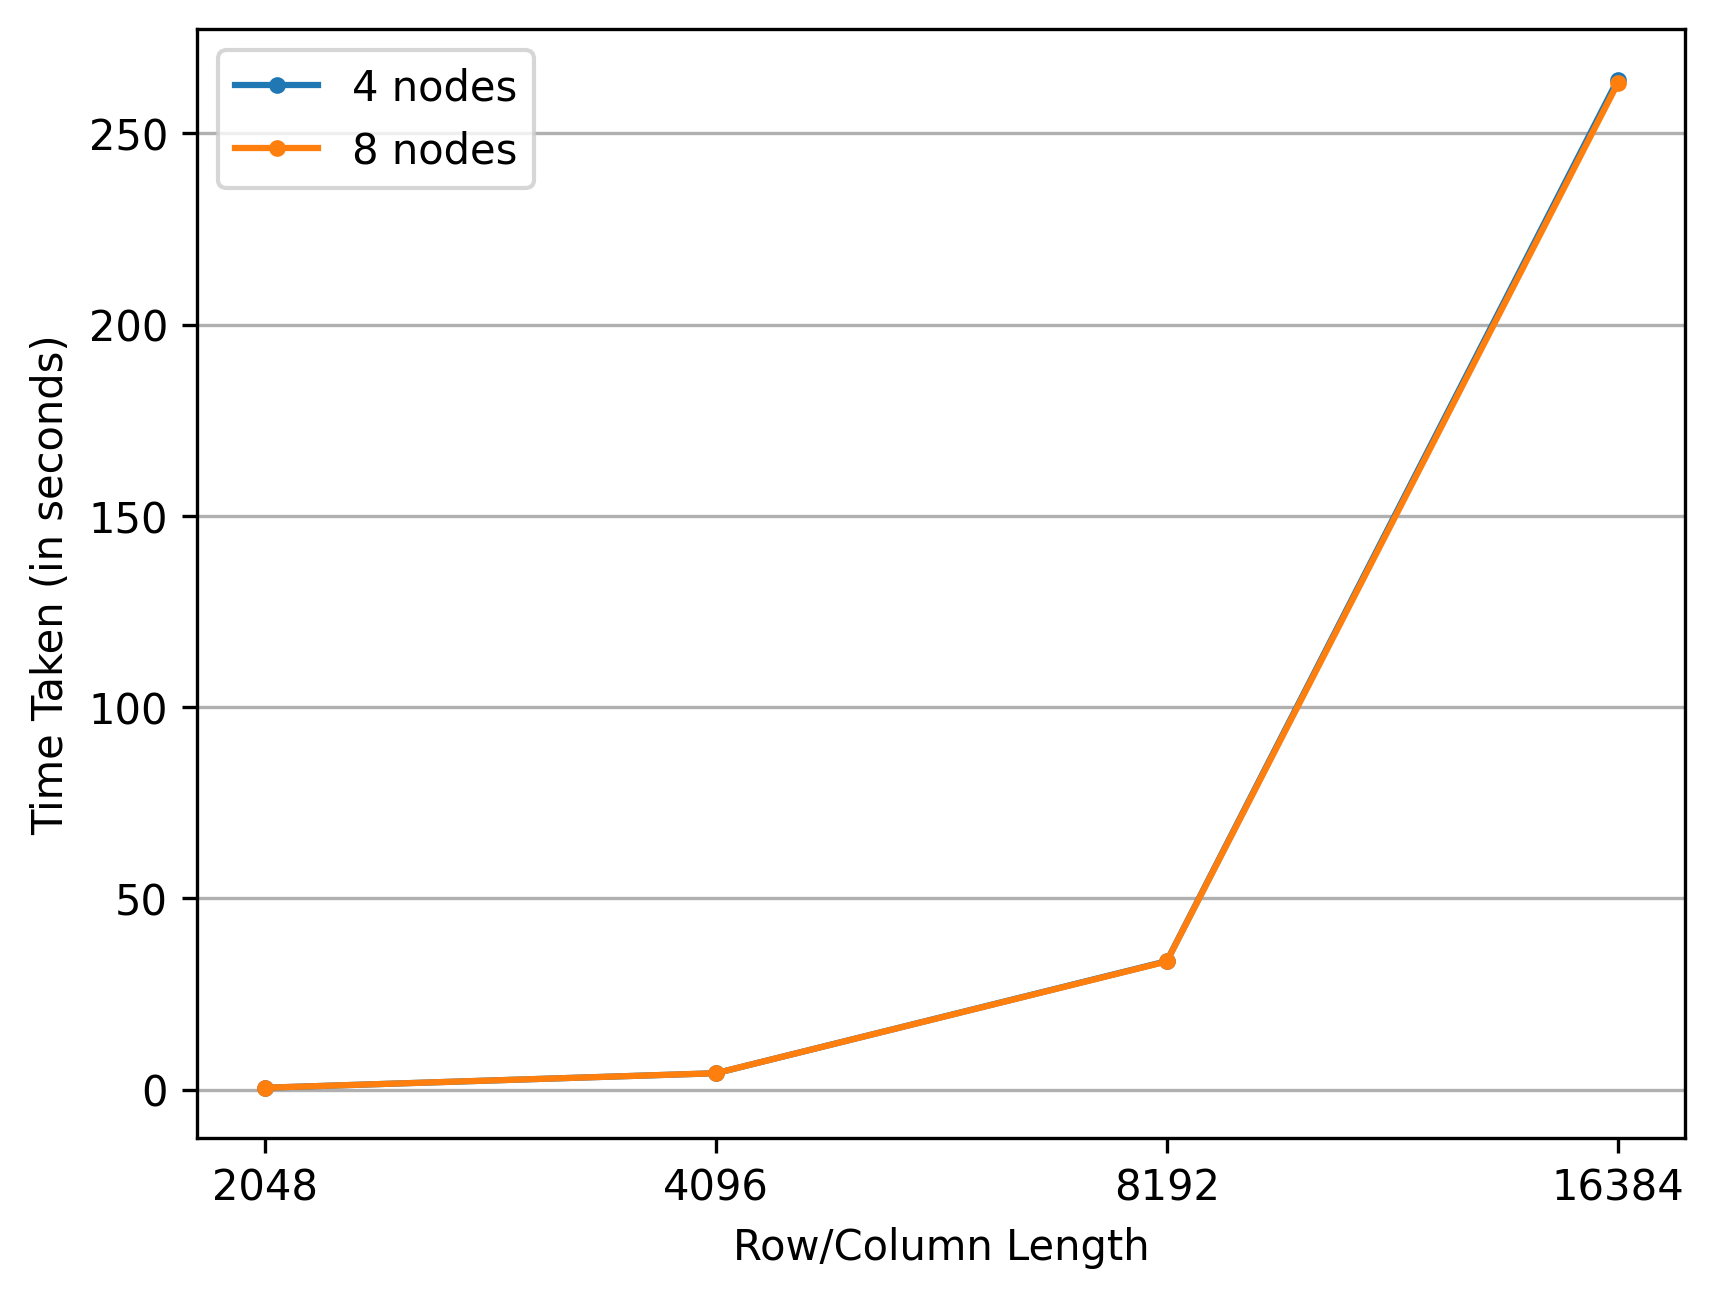
\includegraphics[width=\textwidth]{img/MPI/mpi_strong_scaling.png}
        \caption{Comparison between MPI using 4 or 8 nodes}
        \label{MPI_4_8_NODES}
    \end{minipage}
    \hfill
    \begin{minipage}[t]{0.49\textwidth}
        \centering
        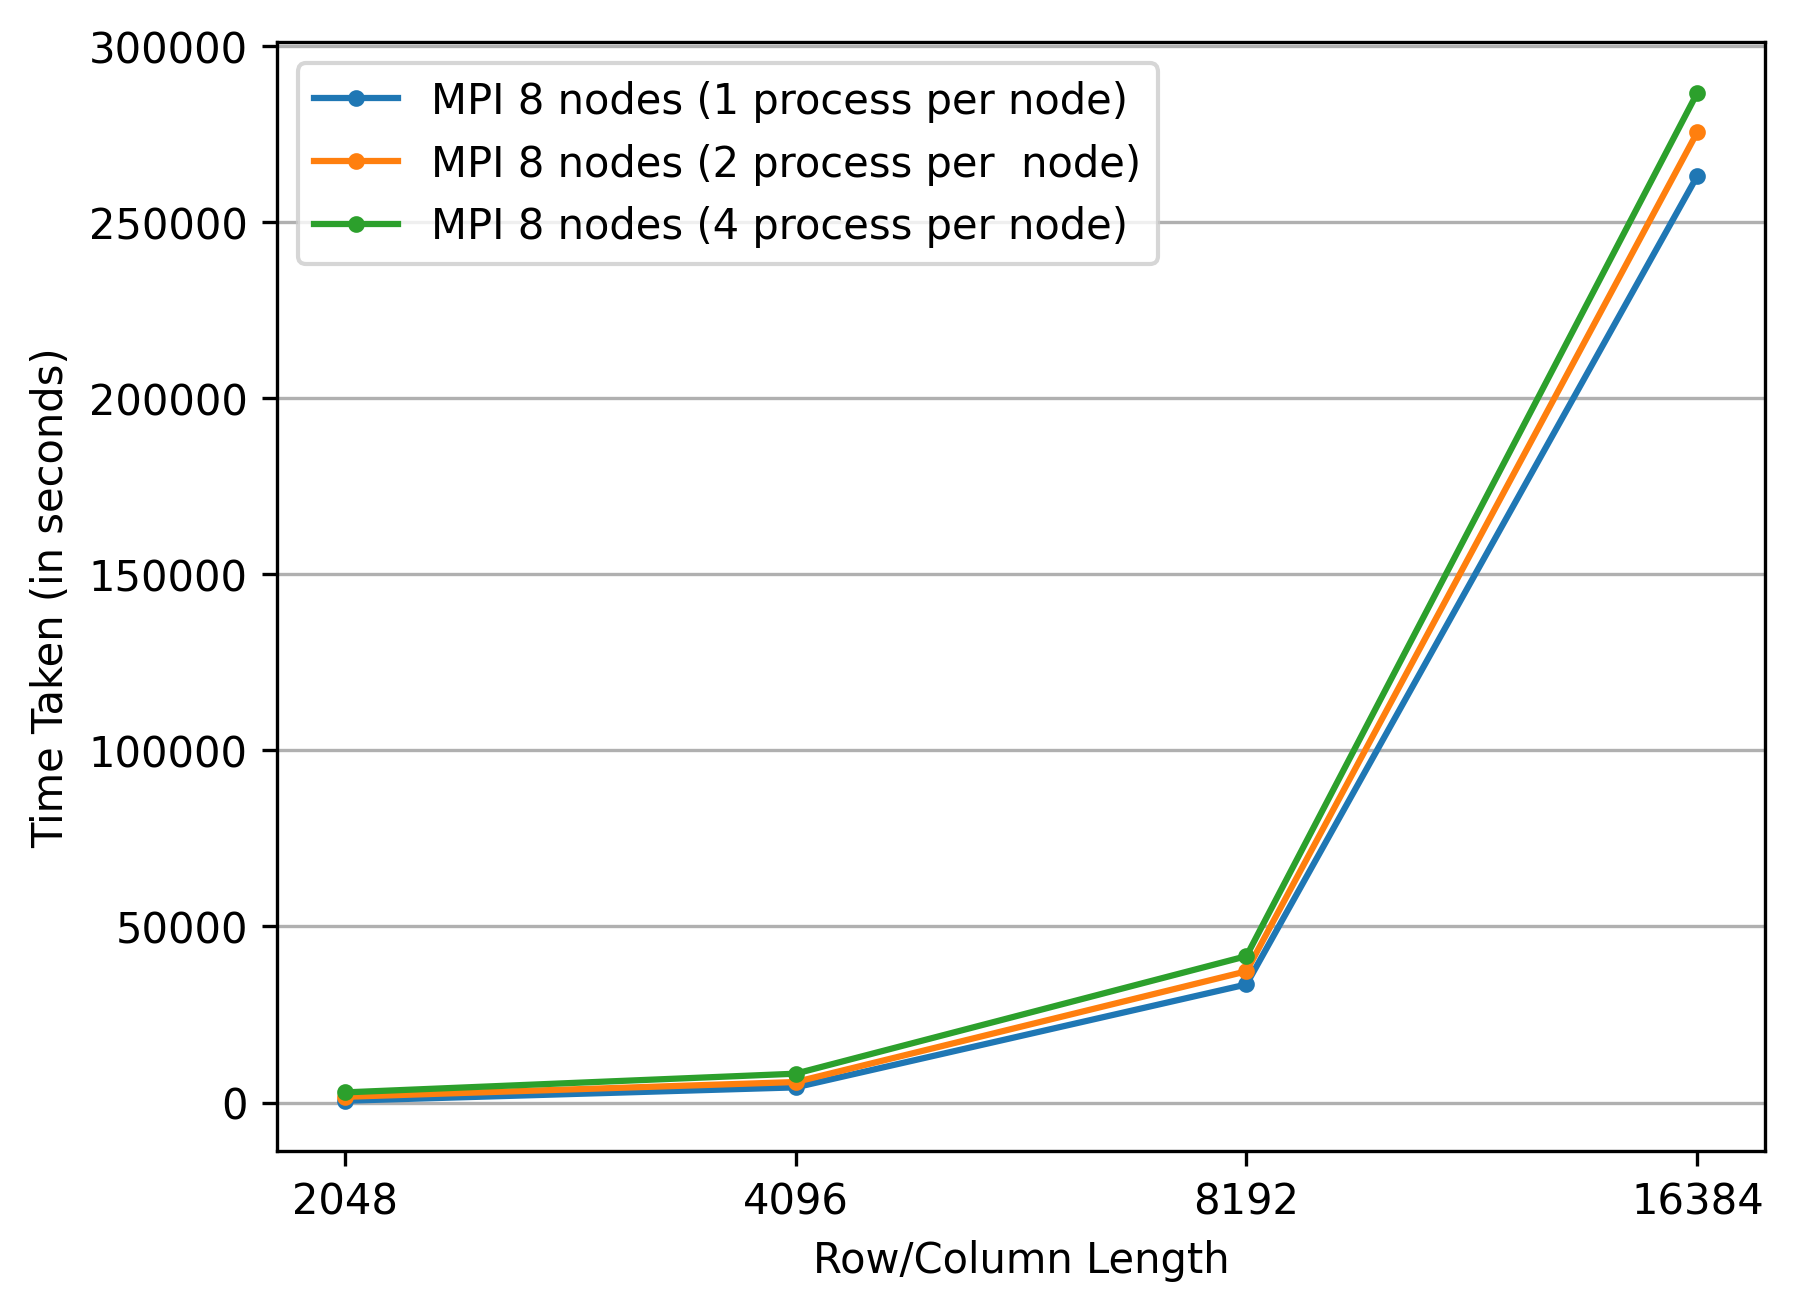
\includegraphics[width=\textwidth]{img/MPI/mpi_threads.png}
        \caption{Comparison giving more threads per node}
        \label{MPI_THEADS}
    \end{minipage}
    
    % First row: Two images adjacent
    \begin{minipage}[t]{0.49\textwidth}
        \centering
        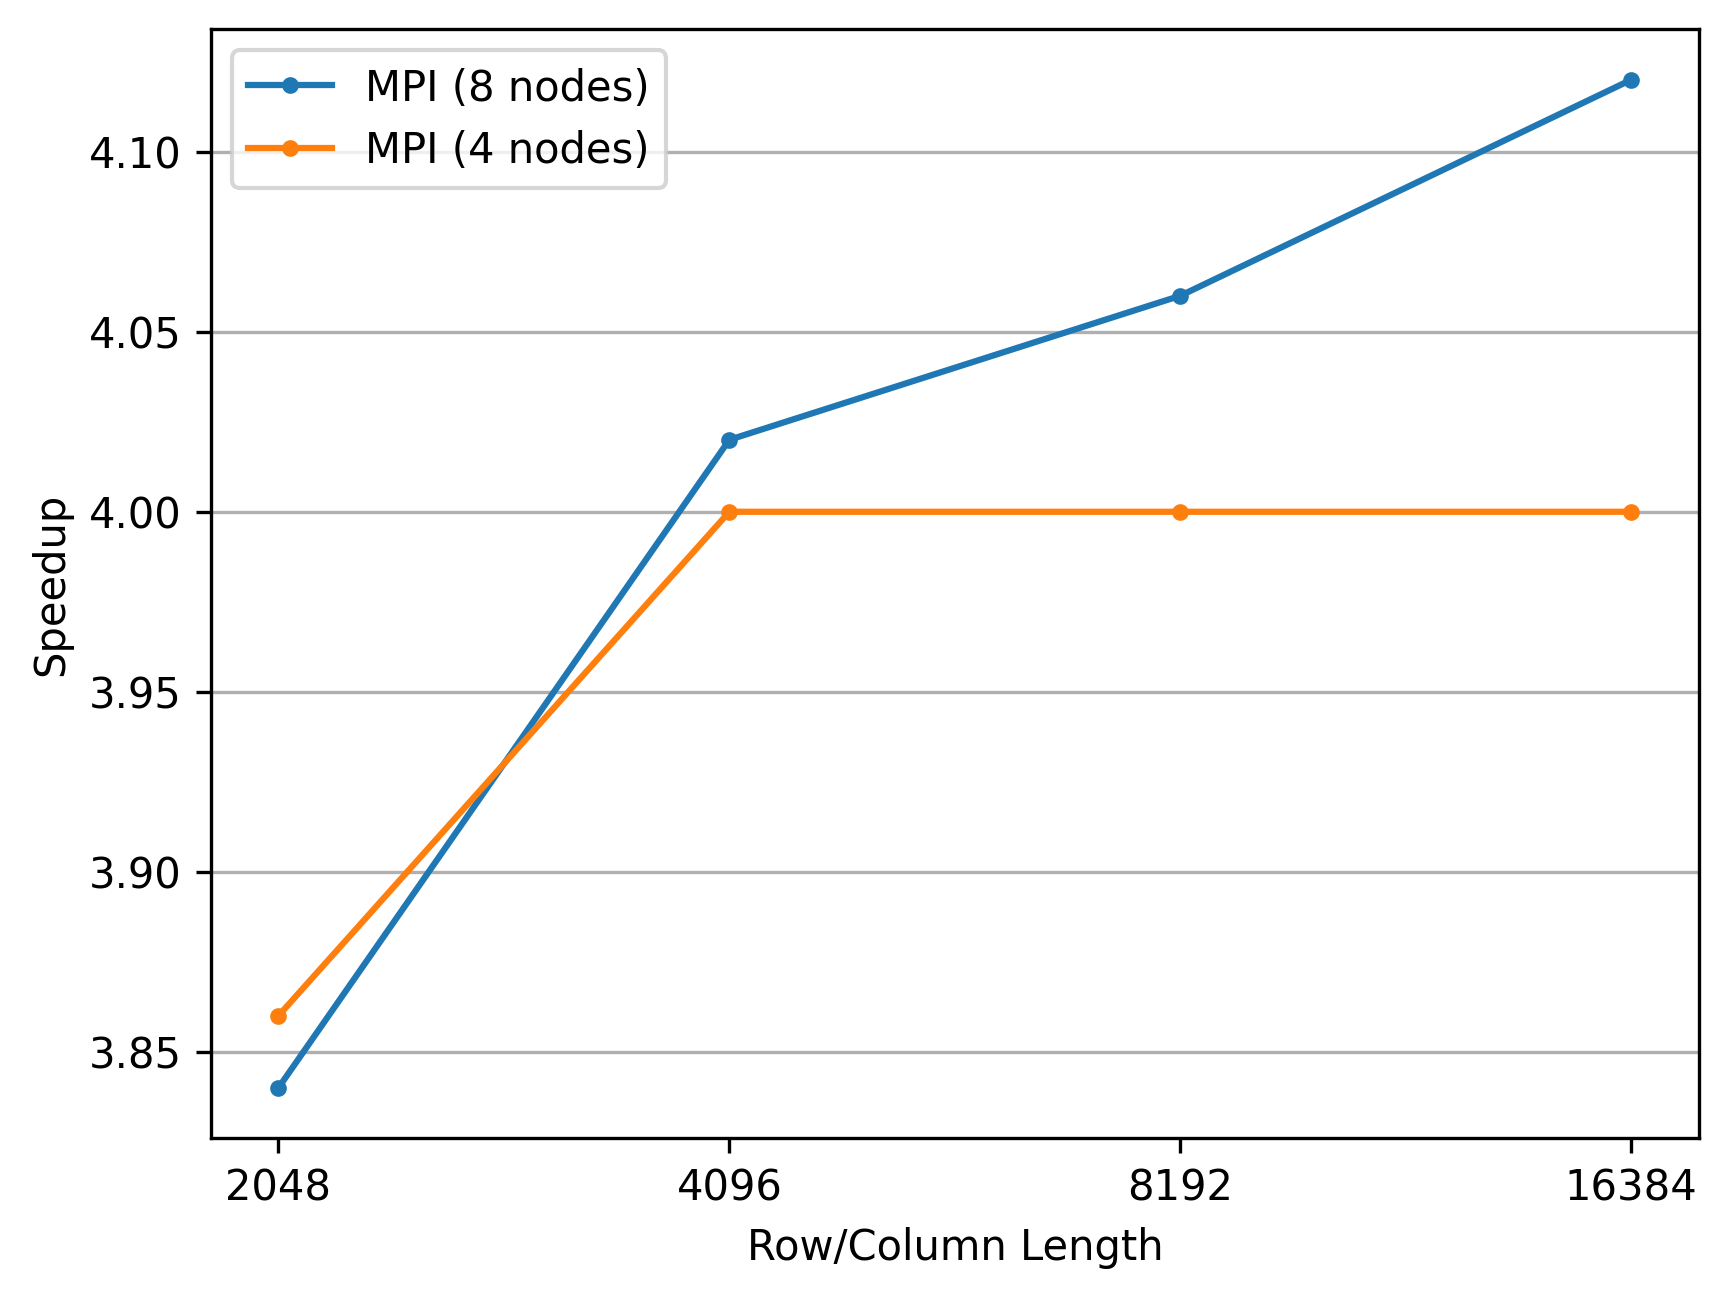
\includegraphics[width=\textwidth]{img/MPI/mpi_speedup.png}
        \caption{Speedup comparison in MPI}
        \label{MPI_Speedup}
    \end{minipage}
    \hfill
    \begin{minipage}[t]{0.49\textwidth}
        \centering
        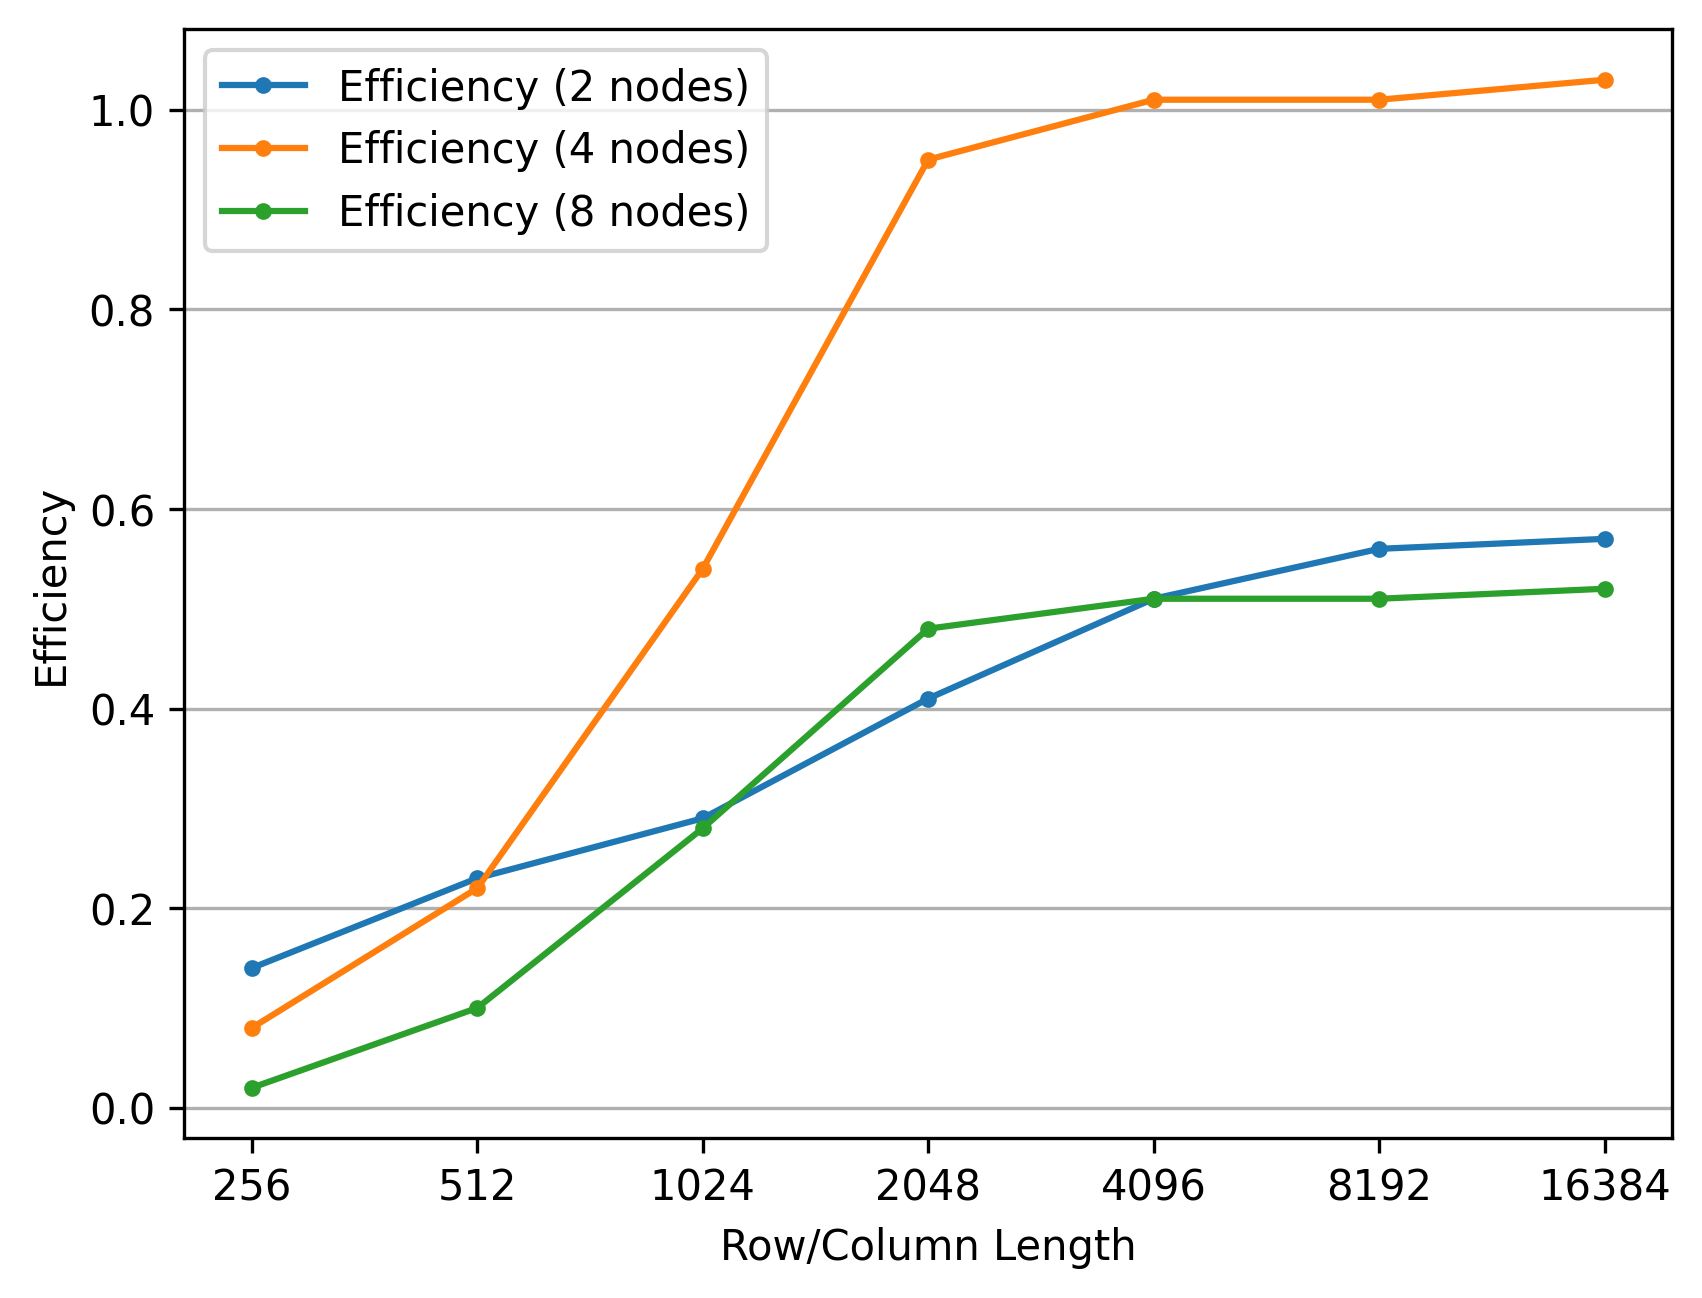
\includegraphics[width=\textwidth]{img/MPI/mpi_efficiency.png}
        \caption{Efficiency comparison in MPI}
        \label{MPI_Efficiency}

    \end{minipage}
    \begin{minipage}[t]{0.90\textwidth}
        \centering
        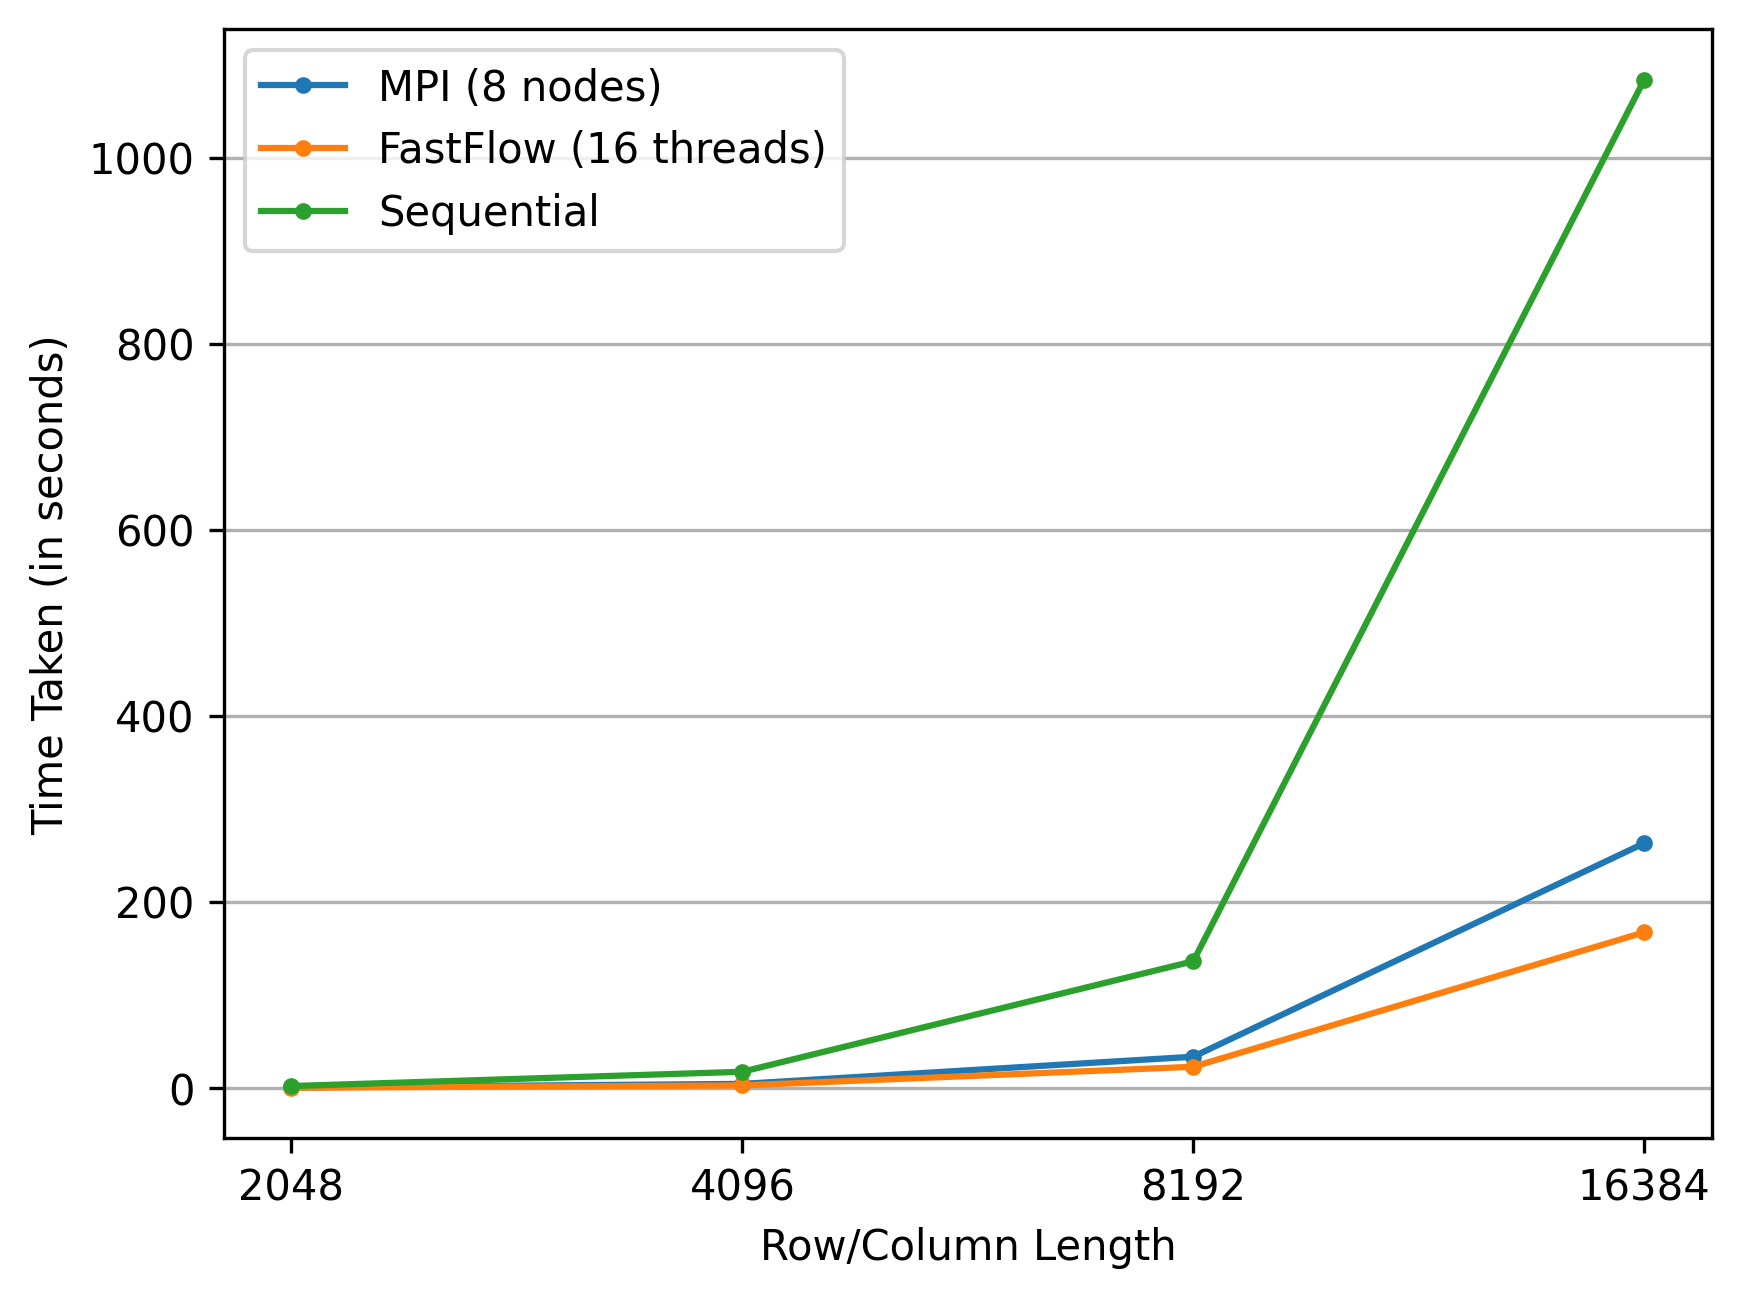
\includegraphics[width=\textwidth]{img/MPI/general_comparison.png}
        \caption{A general comparison between all implementation}
        \label{FF_Chunk}
    \end{minipage}
\end{figure}

\section*{Project Structure}
The project is available on GitHub at the repository: \href{https://github.com/Sallo97/SPM_Project-Wavefront_Pattern}{https://github.com/Sallo97/SPM\_Project-Wavefront\_Pattern}. The root directory includes a CMake file for compiling the project (details provided in the next section), a document describing the project, this report, a README with a brief overview and compilation instructions, and the following folders:

\begin{itemize} 
    \item \textbf{include:} Includes support libraries, specifically the \texttt{FastFlow} library for this project. Before compiling, make sure to run the \textit{``mapping\_string.sh''} script to ensure that \texttt{FastFlow} compiles and optimizes version of the code for the machine used.

    \item \textbf{results:} Stores \texttt{CSV} files containing the average results of each implementation. Each result is organized into subdirectories based on the implementation.

    \item \textbf{scripts:} Contains \texttt{SLURM} scripts used to measure the performance of the implementations in the compute cluster.

    \item \textbf{src:} Contains the source files for the various implementations. Within this directory, the \textit{``utils''} subfolder holds support header files used throughout the project.
\end{itemize}



\subsection*{Compiling and executing the Project}
To compile the entire project, open the terminal at the project's root directory and run the \texttt{cmake} command. It is recommended to keep the build directory separated from the source directory. To do this, use the command \texttt{cmake -B <build\_folder>}, where \texttt{<build\_folder>} is the name of the directory where you want to store the build files. Then, navigate to this build directory and execute \texttt{make} to compile the project. Following these recommendations, the binaries will be stored in the \texttt{src} subfolder. The binaries are the following:
\begin{itemize}
    \item \texttt{sequential [length the matrix]}: execute a sequential implementation of the Wavefront pattern.
    \item \texttt{parallel\_fastflow\_dynamic\_chunk [length of the matrix] [threads to spawn]}: execute the \texttt{FastFlow} implementation of the Wavefront pattern with the given number of threads as node of the Farm. It computes dynamically the chunk size.
    \item \texttt{parallel\_fastflow\_static\_chunk [length of the matrix] [num of threads to spawn]}: execute the \texttt{FastFlow} implementation of the Wavefront pattern with the given number of threads as node of the Farm. It computes dynamically the chunk size.
    \item \texttt{parallel\_mpi [length of the matrix]}: execute the \texttt{MPI} implementation of the Wavefront pattern. Recall that to run the following binary it is needed to call \texttt{mpirun} in the following way: \texttt{mpirun -N [number of nodes to use] ./parallel\_mpi [length of a row of the matrix]}.
\end{itemize}

The \texttt{scripts} folder contains scripts for each implementation, executing them with various matrix lengths (typically from 256 to 16,384) and, where applicable, different numbers of threads or nodes. These scripts were run on the \textit{``spmcluster.unipi.it''} compute cluster to gather the measurements discussed in this report. Each script generates a \texttt{.out} file in the \texttt{results/<implementation>} directory, recording the time for each execution. The average results of the tests done are saved in \texttt{CSV} files in the results folder. 

\section*{Conclusions}
In this report, I explored two distinct approaches to parallelizing the Wavefront pattern: a shared memory solution using the \texttt{FastFlow} library and a distributed memory approach with \texttt{MPI}. Each implementation comes with its own set of advantages and disadvantages, highlighting the fundamental differences in addressing the problem across different architectures. The analysis revealed that the optimal approach depends on the problem's scale. For small matrices (up to 256), a sequential approach is most efficient. As matrix sizes increase, a shared memory solution like \texttt{FastFlow} becomes more effective. However, the matrices we tested are still relatively small and can be comfortably stored within the memory limits of a single process. For much larger matrices, such as those encountered in data centers, a distributed memory approach like \texttt{MPI} becomes essential. The key takeaway is to always record and compare performance measurements to account for overheads, enabling more effective and efficient parallelization strategies.
\end{document}